\documentclass[a4paper,11pt]{book}
%\documentclass[a4paper,twoside,11pt,titlepage]{book}
\usepackage{listings}
\renewcommand{\lstlistingname}{Código}% Listing -> Código
\usepackage[utf8]{inputenc}
% \usepackage[style=list, number=none]{glossary} %
%\usepackage{titlesec}
%\usepackage{pailatino}
\usepackage[spanish]{babel}
\usepackage{amsmath,amssymb,amsthm,mathtools}
\usepackage{mdframed}
\usepackage{lipsum}
\usepackage{dcolumn}
\usepackage{titlesec}
\usepackage{caption}
\usepackage{pgfplots} %% PINTAR
\usepackage{tikz}
\usetikzlibrary{arrows.meta}
\usepackage{verbatim} % comentarios
\graphicspath{{./imagenes/}}
\newcolumntype{.}{D{.}{\esperiod}{-1}}
\makeatletter
\makeatother

%%%%%%%%%% LO QUE YO HE INTRODUCIDO %%%%%%%%%%%%
 % Recuadrar teorema/lema y asignarlo a un capítulo
\newmdtheoremenv{teoremaBox}{Teorema}[chapter]
\newmdtheoremenv{lemaBox}{Lema}[chapter]
\newmdtheoremenv{proposicionBox}{Proposición}[chapter]
\newmdtheoremenv{corolarioBox}{Corolario}[chapter]

\newtheorem{observacion}{Observación}[chapter]
 % Usar recuadro negro el terminar demostración
\renewcommand\qedsymbol{$ \blacksquare $}
%\renewcommand\proof{\textit{Demostración:}  \qedsymbol}

% EVITAR QUE PONGA "CHAPTER *" AL INICIO DEL CAPÍTULO
\titleformat{\chapter}[display]{\normalfont\bfseries}{}{0pt}{\Huge}

\def\spanishoperators{adj traza vect dom dist sop vol sgn  Hess Jac rango grado diag img longitud Maximizar Minimizar Optimizar sec cotan cosec}
\newcommand{\refPar}[1]{(#1)}
\newcommand{\w}{\displaystyle}
\newcommand{\norm}[1]{\left\Vert#1\right\Vert}
\newcommand{\abs}[1]{\left\vert#1\right\vert}
\newcommand{\pre}[1]{\left\langle#1\right\rangle}
\newcommand{\set}[1]{\left\{#1\right\}}
\newcommand{\RR}{\mathbb{R}}
\newcommand{\NN}{\mathbb{N}}
\newcommand{\ZZ}{\mathbb{Z}}
\newcommand\restr[2]{{% ejemplo: \restr{f}{A}
		\left.\kern-\nulldelimiterspace #1 \vphantom{\big|} \right|_{#2} 
}}

\newcommand{\vecN}[2][N]{$\{{#2}_{1},...,{#2}_{#1} \}$ }
\newcommand{\vecSpace}{ $V$ }

%%%%%%%%%%%%%%%%%%%%%%%%%%%%%%%%%%%%%%%%%%%%%%%%%%%%%%%%%%%%%%

%\usepackage[chapter]{algorithm}
\RequirePackage{verbatim}
%\RequirePackage[Glenn]{fncychap}
\usepackage{fancyhdr}
\usepackage{graphicx}
\usepackage{afterpage}

\usepackage{longtable}

\usepackage[pdfborder={000}]{hyperref} %referencia

% ********************************************************************
% Re-usable information
% ********************************************************************
\newcommand{\myTitle}{Título del proyecto\xspace}
\newcommand{\myDegree}{Grado en ...\xspace}
\newcommand{\myName}{Nombre Apllido1 Apellido2 (alumno)\xspace}
\newcommand{\myProf}{Nombre Apllido1 Apellido2 (tutor1)\xspace}
\newcommand{\myOtherProf}{Nombre Apllido1 Apellido2 (tutor2)\xspace}
%\newcommand{\mySupervisor}{Put name here\xspace}
\newcommand{\myFaculty}{Escuela Técnica Superior de Ingenierías Informática y de
Telecomunicación\xspace}
\newcommand{\myFacultyShort}{E.T.S. de Ingenierías Informática y de
Telecomunicación\xspace}
\newcommand{\myDepartment}{Departamento de ...\xspace}
\newcommand{\myUni}{\protect{Universidad de Granada}\xspace}
\newcommand{\myLocation}{Granada\xspace}
\newcommand{\myTime}{\today\xspace}
\newcommand{\myVersion}{Version 0.1\xspace}


\hypersetup{
pdfauthor = {\myName (email (en) ugr (punto) es)},
pdftitle = {\myTitle},
pdfsubject = {},
pdfkeywords = {palabra_clave1, palabra_clave2, palabra_clave3, ...},
pdfcreator = {LaTeX con el paquete ....},
pdfproducer = {pdflatex}
}

%\hyphenation{}


%\usepackage{doxygen/doxygen}
%\usepackage{pdfpages}
\usepackage{url}
\usepackage{colortbl,longtable}
\usepackage[stable]{footmisc}
%\usepackage{index}

%\makeindex
%\usepackage[style=long, cols=2,border=plain,toc=true,number=none]{glossary}
% \makeglossary

% Definición de comandos que me son tiles:
%\renewcommand{\indexname}{Índice alfabético}
%\renewcommand{\glossaryname}{Glosario}

\pagestyle{fancy}
\fancyhf{}
\fancyhead[LO]{\leftmark}
\fancyhead[RE]{\rightmark}
\fancyhead[RO,LE]{\textbf{\thepage}}
\renewcommand{\chaptermark}[1]{\markboth{\textbf{#1}}{}}
\renewcommand{\sectionmark}[1]{\markright{\textbf{\thesection. #1}}}

\setlength{\headheight}{1.5\headheight}

\newcommand{\HRule}{\rule{\linewidth}{0.5mm}}


%Definimos los tipos teorema, ejemplo y definición podremos usar estos tipos
%simplemente poniendo \begin{teorema} \end{teorema} ...
\newtheorem{teorema}{Teorema}[chapter]
\newtheorem{ejemplo}{Ejemplo}[chapter]
\newtheorem{definicion}{Definición}[chapter]

\definecolor{gray97}{gray}{.97}
\definecolor{gray75}{gray}{.75}
\definecolor{gray45}{gray}{.45}
\definecolor{gray30}{gray}{.94}

\lstset{ frame=Ltb,
     framerule=0.5pt,
     aboveskip=0.5cm,
     framextopmargin=3pt,
     framexbottommargin=3pt,
     framexleftmargin=0.1cm,
     framesep=0pt,
     rulesep=.4pt,
     backgroundcolor=\color{gray97},
     rulesepcolor=\color{black},
     %
     stringstyle=\ttfamily,
     showstringspaces = false,
     basicstyle=\scriptsize\ttfamily,
     commentstyle=\color{gray45},
     keywordstyle=\bfseries,
     %
     numbers=left,
     numbersep=6pt,
     numberstyle=\tiny,
     numberfirstline = false,
     breaklines=true,
   }
 
% minimizar fragmentado de listados
\lstnewenvironment{listing}[1][]
   {\lstset{#1}\pagebreak[0]}{\pagebreak[0]}

\lstdefinestyle{CodigoC}
   {
	basicstyle=\scriptsize,
	frame=single,
	language=C,
	numbers=left
   }
\lstdefinestyle{CodigoC++}
   {
	basicstyle=\small,
	frame=single,
	backgroundcolor=\color{gray30},
	language=C++,
	numbers=left
   }

 
\lstdefinestyle{Consola}
   {basicstyle=\scriptsize\bf\ttfamily,
    backgroundcolor=\color{gray30},
    frame=single,
    numbers=none
   }


\newcommand{\bigrule}{\titlerule[0.5mm]}


%Para conseguir que en las páginas en blanco no ponga cabecerass
\makeatletter
\def\clearpage{%
  \ifvmode
    \ifnum \@dbltopnum =\m@ne
      \ifdim \pagetotal <\topskip
        \hbox{}
      \fi
    \fi
  \fi
  \newpage
  \thispagestyle{empty}
  \write\m@ne{}
  \vbox{}
  \penalty -\@Mi
}
\makeatother

\usepackage{pdfpages}
\begin{document}
	\begin{titlepage}
 
 
\newlength{\centeroffset}
\setlength{\centeroffset}{-0.5\oddsidemargin}
\addtolength{\centeroffset}{0.5\evensidemargin}
\thispagestyle{empty}

\noindent\hspace*{\centeroffset}\begin{minipage}{\textwidth}

\centering

\includegraphics[width=0.9\textwidth]{imagenes/logo_ugr.jpg}\\[1.4cm]

\textsc{ \Large TRABAJO FIN DE GRADO\\[0.2cm]}
\textsc{ DOBLE GRADO EN INGENIERÍA EN INGENIERÍA INFORMÁTICA Y MATEMÁTICAS}\\[1cm]
% Upper part of the page
% 
% Title
{\Huge\bfseries Titulo del Proyecto\\
}
\noindent\rule[-1ex]{\textwidth}{3pt}\\[3.5ex]
{\large\bfseries Subtitulo del Proyecto}
\end{minipage}

\vspace{2.5cm}
\noindent\hspace*{\centeroffset}\begin{minipage}{\textwidth}
\centering

\textbf{Autor}\\ {Pedro Manuel Flores Crespo (alumno)}\\[2.5ex]
\textbf{Directores}\\
{Manuel Ruíz Galán (tutor1)\\
Juan Carlos Torres Cantero (tutor2)}\\[2cm]

\includegraphics[width=0.3\textwidth]{imagenes/etsiit_logo.png}\\[0.1cm]
\textsc{Escuela Técnica Superior de Ingenierías Informática y de Telecomunicación}\\
\textsc{---}\\
Granada, mes de 201
\end{minipage}
%\addtolength{\textwidth}{\centeroffset}
%\vspace{\stretch{2}}
\end{titlepage}



%\frontmatter
\tableofcontents
%\listoffigures
%\listoftables
%
%\mainmatter
%\setlength{\parskip}{5pt}

\chapter{Resumen y palabras clave}

El trabajo fin de grado que presentamos supone la incursión a un campo dentro de la optimización, los teoremas de la alternativa, y sus aplicaciones, principalmente a la propia optimización y finanzas. El trabajo comienza con el teorema de Mazur-Orlicz-König, versión del conocido teorema de Hahn-Banach. Posteriormente, estudiamos el teorema de la alternativa de Gordan, esencial para el resto de resultados. Su primera aplicación se da en la teoría minimax, que nos conduce a resultados clásicos sobre separación de convexos. A continuación, deduciremos otro teorema de la alternativa, el de Farkas, y lo aplicaremos a la programación lineal. Para demostrar los resultados sobre optimización, volvemos al teorema de Gordan, que nos proporcionara los teoremas de Fritz John y Karush-Kuhn-Tucker. Finalmente, nos introducimos en el mundo de las matemáticas financieras obteniendo, gracias al teorema de separación, el primer teorema de asignación de precios para valorar opciones europeas. Concluimos realizando simulaciones de su valor en diferentes casos.\\

% Keywords command
\providecommand{\pclave}[1]
{
	\small	
	\textbf{\textit{Palabras clave: }} #1
}
\pclave{teoremas de la alternativa, teorema de Hahn-Banach, minimax, optimización, matemáticas financieras.}
\chapter{Resumen extendido y palabras clave en inglés}
The end of degree project that we present is an incursion into a field included in optimization, the theorems of the alternative, and their applications, mainly to the own optimization and finances.\\

Many of the theorems of the alternative are just reformulations of convex separation's theorems in certain contexts, so we start this memory with a study on Hahn-Banach's theorem. There are several equivalent versions of this result, collected for example in \cite{schechter1996handbook}. That is the reason why many authors talk about Hahn-Banach's theorems. We will focus on one of them, Mazur-Orlicz-König's theorem. Despite its geometrical charge, tt is mainly an algebraical result. We will provide a proof of that theorem -- the results in this work are self-contained --  and we will use it to give a convex version  of Gordan's theorem of alernative. Actually, it is an equivalent result due to S. Simons. This version is more general than the orginal Gordan's result and it will be extremmely useful in the next important results. \\

Then, we will apply the convex Gordan's theorem of the alternative in the minimax theory. A minimax inequality guarantees, under certain hypothesis, that in a two variables function we can substitute inf\hspace{0.5mm}sup for sup\hspace{0.5mm}inf. The power of minimax inequalities is clear when we use it -- in one that we will deduce from the convex Gordan's theorem -- to give classical convex separation's results. \\

Next, we will deduce from one separation's theorem the Farkas's lemma, which is one of the most known theorem of the alternative. This will allow us to prove, almost immediately, one of the key points of linear programming: the duality theorem. Considering more general optimization theorems, those in which the objective function and the inequalities constraints are differentiables, we wil establish, using Gordan's theorem of the alternative, the theorems of Fritz John and Karush-Kuhn-Tucker.\\

We will conclude with a little foray into the field of financial mathematics. After introducing some of the main concepts, like a derivate security; we will prove, as a consequence of one of the convex separation's theorem, the result kwonw as ``First Fundamental Theorem of Asset Pricing''. It can be used in the pricing of European's options in the binomial model. Finally, we have programmed using \textit{Sagemath 2.8} some examples in order to know how their price varies according to its parametres.\\

% Keywords command
\providecommand{\keywords}[1]
{
	\small	
	\textbf{\textit{Keywords: }} #1
}
\keywords{theorems of the alternative, Hahn-Banach's theorem, minimax, optimization, financial mathematics.}
\input{capitulos/Introducción.tex}
\chapter{Objetivos}
Los objetivos inicialmente previstos en la propuesta de TFG fueron:
\begin{itemize}
\item Realizar una recopilación de algunos teoremas de la alternativa.
\item Teorema de dualidad en programación lineal.
\item Teoremas de Karush-Kuhn-Tucker y Fritz John para programación convexa.
\item Aplicación a finanzas: teorema fundamental de valoración de activos financieros en mercados finitos.
\end{itemize}

Sin embargo, nuestro tratamiento final ha sido algo más ambicioso, pues hemos incluido todo un capítulo de aplicaciones de los teoremas de la alternativa a la teoría minimax y a la separación de convexos. Además, en lugar de considerar los teoremas de Karush-Kuhn-Tucker y Fritz John en un ambiente convexo, los hemos establecido en un contexto no lineal y diferenciable. La idea que nos ha llevado a ello ha sido aumentar el número y tipología de aplicaciones de los teoremas de la alternativa, mostrando su versatilidad en diversos campos.
\chapter{Desarrollo}
El proceso seguido en el desarrollo del TFG ha sido, por un lado, recopilar material sobre el tema y analizarlo, y por otro, darle estructura totalmente autocontenida, elaborando los diversos contenidos de forma jerarquizada en el sentido de que se deducen de los anteriores. A modo de esquema, los resultados se han estructurado atendiendo al siguiente esquema donde además se recoge la relación entre ellos: 
\begin{figure}[h!]
	\centering
	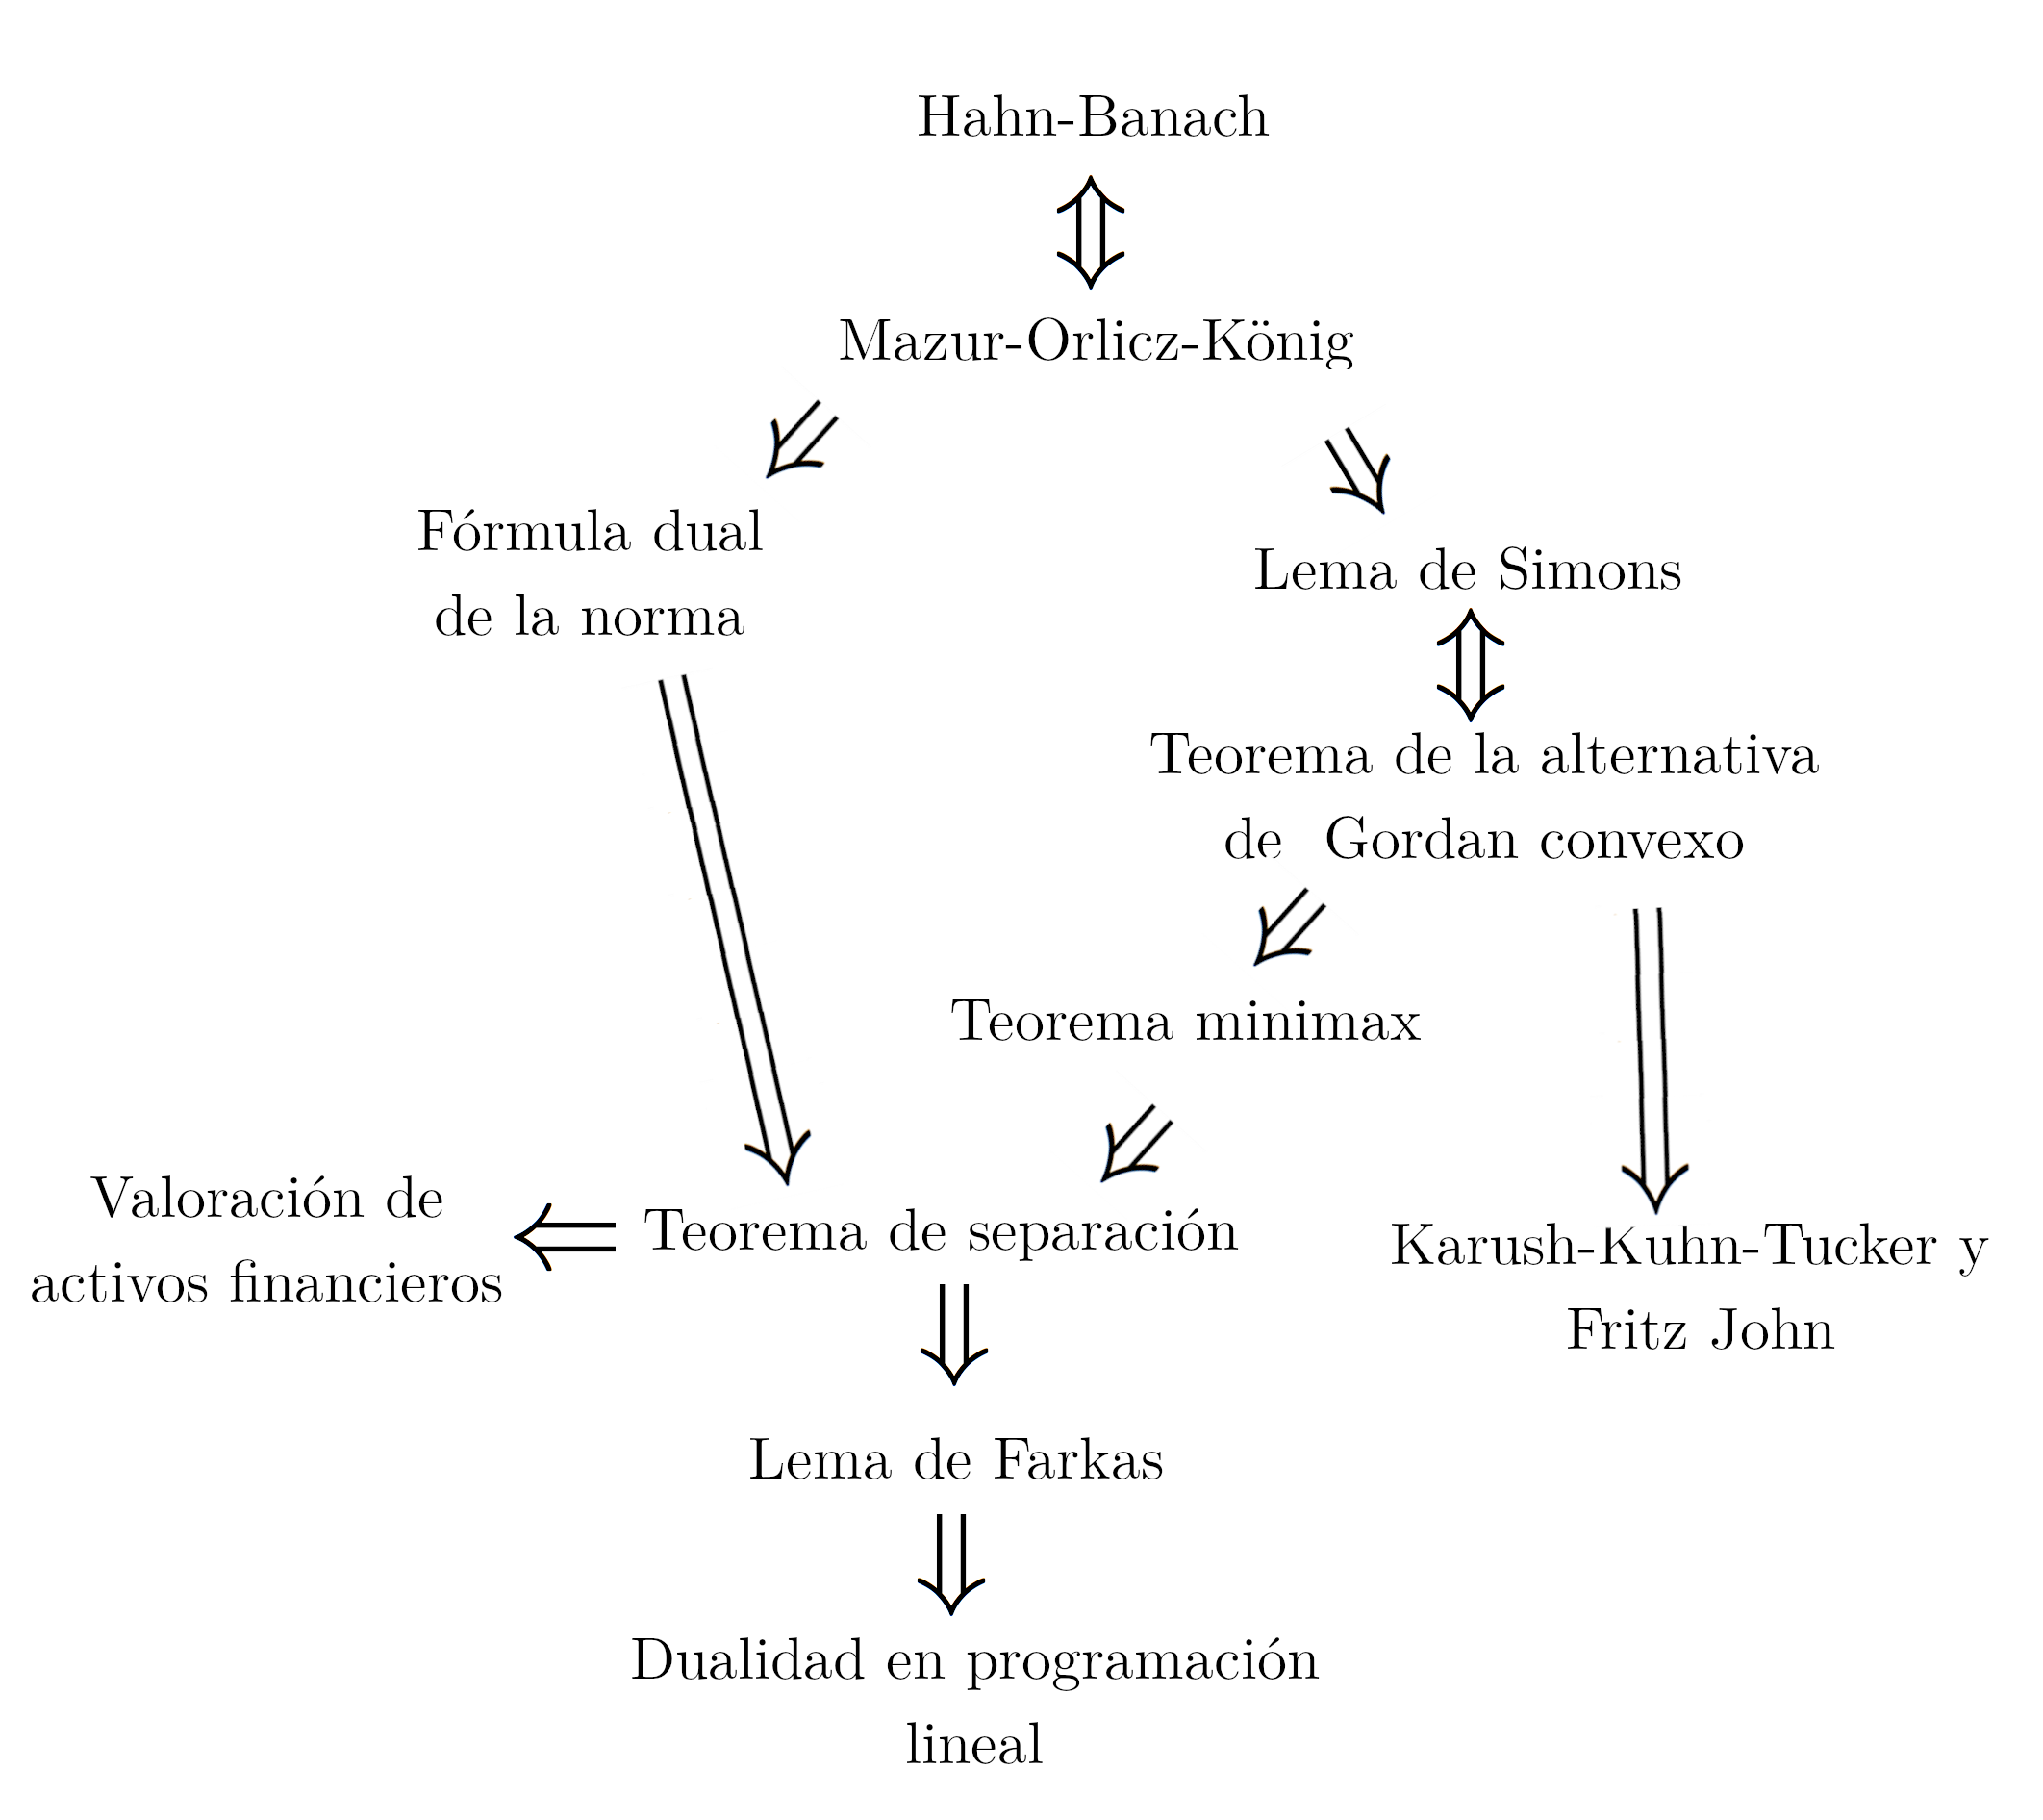
\includegraphics[width=0.9\linewidth]{imagenes/esquema.png}
	\label{fig:aux2}
\end{figure}

Como puede observarse, las técnicas son de carácter convexo y analítico funcional.
\\

\chapter{Teoremas de la alternativa}
Los teoremas de la alternativa constituyen una potente herramienta en optimización. A pesar de tener un claro carácter convexo, se aplican incluso a problemas no convexos, tal y como se comprobará a lo largo de esta memoria. Nuestro punto de partida es el resultado del análisis  convexo, más importante, el teorema de Hahn-Banach. Es más, daremos una versión equivalente debida a H. König, conocida como el teorema de Mazur-Orlicz-König. Como consecuencia, obtendremos el teorema de la alternativa de Gordan, tanto en su versión convexa como una más general. 

\section{Teorema de Mazur-Orlicz-König}
El objetivo principal de esta sección es demostrar una versión equivalente no muy conocida del clásico teorema de Hanh-Banach, el teorema de Mazur-Orlicz-König. Iremos de una versión básica y algebraica del teorema de Hahn-Banach al teorema de Mazur-Orlicz-König siguiendo como aparece en el texto de S. Simons \cite{Simons2008}. \\
	
En primer lugar vamos a recordar la definición de funcional sublineal sobre un espacio vectorial \vecSpace . Notar que todos los espacios vectoriales que vamos a usar son reales. Del mismo modo, los espacios y conjuntos que usaremos asumiremos que son no vacíos.
	
\begin{definicion}
Sea \vecSpace un espacio vectorial. Decimos que el $P:\vecSpace \rightarrow \RR$ es sublineal si cumple las siguientes condiciones:
	\begin{itemize}
		\item $ P $ es subaditiva: $x_1, x_2 \in \vecSpace \Longrightarrow P(x_1 + x_2) \leq P(x_1) + P(x_2) $.
		\item $ P $ es positivamente homogénea: $x_1 \in \vecSpace $ y $ \lambda > 0 \Longrightarrow P(\lambda x) = \lambda P(x) $.
	\end{itemize}
\end{definicion}

Como consecuencia, podemos afirmar que $ P(0) = 0 $. En efecto:
\[
P(0) = P(2\times0) = 2\times P(0) \Longrightarrow P(0) = 0.
\]

Por ejemplo, toda norma o incluso toda seminorma sobre \vecSpace es un funcional sublineal. Así, dados $ a,b \in \RR $ con $ a <b $ tenemos que $ P:H^{1} (a,b) \longrightarrow \RR$ definida como \[ P(x) = \norm{x'}_{L^2(a,b)} \] es una seminorma y por ello sublineal. También, si $ \vecSpace = \RR $ y definimos la parte positiva \[ P(x) = [x]^{+} = \max \{0,x\}, \forall x \in \RR \] obtenemos un funcional sublineal sobre $\RR$. \\
	
El lema que exponemos a continuación, y que generalizaremos posteriormente en el lema \ref{lema2}, nos servirá para demostrar el teorema de Hanh-Banach. 
	
\bigskip
	\begin{lemaBox}\label{lema1}
		Sea\vecSpace un espacio vectorial y $P:\vecSpace \rightarrow \RR$ un funcional sublineal. Fijamos un elemento $ y \in \vecSpace $ y para todo $ x \in \vecSpace $ tomamos  
		\begin{center}
			$ P_y(x) := \displaystyle\inf_{\lambda > 0} \left[P(x+\lambda y) - \lambda P(y)\right] $
		\end{center}
		
		Entonces, $ P_y(\vecSpace) \subset \RR$, $ P_y:\vecSpace \longrightarrow \RR $ es sublineal, $ P_y \leq P $ y además $ P_y (-y) \leq  -P(y)$.
	\end{lemaBox} 
	\begin{proof}
		Fijamos $ y \in V $. Sea $ x \in V $ y $ \lambda > 0$. Como P es sublineal tenemos: 
		\begin{center}
			$ \lambda P(y) = P(\lambda y) =P(\lambda y +x-x) \leq P(x+\lambda y)+ P(-x)$.
		\end{center}
		Por lo tanto, se obtiene que $ P(x+\lambda y) - \lambda P(y) \geq -P(-x) $.  Tomando el ínfimo sobre $ \lambda >0 $ llegamos a $ P_{y}(x)\geq -P(-x) > -\infty$. Por consiguiente, $ P_y(\vecSpace) \subset \RR$, esto es $ P_y:\vecSpace \longrightarrow \RR $. \\
		
		Probaremos ahora que $ P_y $ es sublineal. Empezamos viendo la subaditividad. Tomamos $ x_1, x_2 \in V $ y sean $ \lambda_1, \lambda_2 > 0$ arbitrarios. Entonces, la definición de $ P_y $ da 
		\begin{equation*}
		\begin{split}
		( P(x_1 + \lambda_1 y) - \lambda_1 P(y) ) &+ ( P(x_2 + \lambda_2 y) - \lambda_2 P(y) ) \\
		& \geq ( P(x_1 + x_2 + (\lambda_1+\lambda_2)y)) - (\lambda_1+\lambda_2) P(y) \\
		&\geq P_y (x_1 + x_2 ).
		\end{split}
		\end{equation*}
		Tomando ínfimos sobre $ \lambda_1 $ y $ \lambda_2 $, $  P_y (x_1)  + P_y (x_2 ) \geq P_y (x_1 + x_2 ) $. Así, $ P_y $ es subaditiva. Para comprobar que es positivamente homogénea tomamos $ x \in V $ y $ \mu > 0 $. Entonces:
		\begin{equation*}
		\begin{split}
		P_y (\mu x) &= \inf_{\lambda > 0} \left[P(\mu x+\lambda y) - \lambda P(y)\right] \\
		&= \mu \inf_{\lambda > 0} \left[P(x+ (\lambda / \mu) y) - (\lambda / \mu) P(y)\right] \\
		&= \mu \inf_{\upsilon > 0} \left[P(x+ \upsilon y) - \upsilon  P(y)\right] \\
		&= \mu P_y (x).
		\end{split}
		\end{equation*}	
		Obtenemos que $ P_y $ es positivamente homogénea y como consecuencia sublineal. \\
		
		Para demostrar que $ P_y \leq P $, sea $ x \in V $ y tomando $ \lambda = 1 $ en la definición de $ P_y $,
		\[ P_y(x) \leq P(x+y) - P(y) \leq P(x)+ P(y) - P(y) = P(x) \]
		Como $ x \in \vecSpace $ es arbitrario, entonces $ P_y \leq P $. Finalmente, razonando de manera similar,
		\[P_y(-y) \leq P(-y+y) - P(y) = -P(y).  \]
		
	\end{proof}
\bigskip
El teorema de Hahn-Banach que hemos mencionado antes (básico y algebraico) se enuncia en estos términos:

\bigskip
	\begin{teoremaBox}[Hanh-Banach]\label{H-B}
		Sea V un espacio vectorial y $P:V \rightarrow \RR$ un funcional sublineal. Entonces existe un funcional lineal $ L:\vecSpace \longrightarrow \RR $ tal que $ L \leq P $.
	\end{teoremaBox}
\begin{figure}[h!]
	%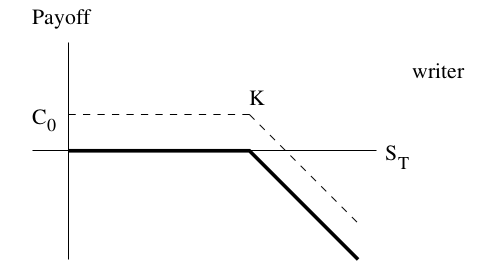
\includegraphics[width=1\linewidth]{Writer_call}
	\centering
	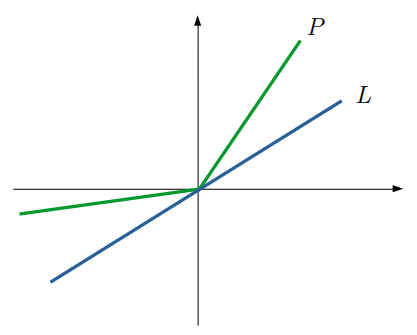
\includegraphics[width=0.6\linewidth]{H-B}
	\caption{Teorema de Hahn-Banach.}
\end{figure}

	\begin{proof}
		Sea $ \text{SUB} = \lbrace Q:\vecSpace \longrightarrow \RR : Q \leq P \rbrace$, es decir, el conjunto de funcionales sublineales sobre \vecSpace que minoren a $ P $. Nuestro propósito es emplear el lema de Zorn con objeto de probar que tiene un elemento minial y tal elemento será el funcional $ L $ que buscamos. Para ello, dados $ T_1 ,T_2 \in \text{SUB} $ consideramos la relación de orden usual, es decir:
		\begin{center}
			$ T_1 \leq T_2 \Longleftrightarrow T_1 (x) \leq T_2 (x) \quad \forall x \in \vecSpace $.
		\end{center}
		Primero probaremos que todo subconjunto $ \mathcal{T} $ totalmente ordenado de $SUB $ tiene una cota inferior en  SUB. Definimos $ Q(x):=\inf \{ T(x): T \in \mathcal{T} \} $ y queremos ver que $ Q(x) \in \RR $. Si $ x \in \vecSpace $ y $ T \in \mathcal{T} $, como T es subaditiva obtenemos la siguiente relación:
		\[ 0 = T(0) = T(x-x) \leq T(x) + T(-x) \Longrightarrow T(x) \geq -T(-x) \quad (1)\]  
		Por otro lado:
		\[ T \in \mathcal{Q} \Longrightarrow T(x) \leq P(x) \Longrightarrow -T(x) \geq -P(x) \quad (2)\] 
		Usando (1), (2) y tomando ínfimo sobre $  T $  llegamos a $ Q(x) \geq -P(x) \geq - \infty $. Por lo tanto $ Q:V \rightarrow \RR$. \\
		
		Ahora probaremos que $ Q $ es subaditiva. Para ello, tomamos $ x_1, x_2\in \vecSpace $. Sean $ T_1 , T_2 \in \mathcal{T} $ arbitrarios. Si $ T_1 \geq T_2 $ (el caso de $ T_2 \geq T_1 $ es análogo.):
		
		\begin{center}
			$ T_1 (x_1)+  T_2 (x_2) \geq T_2(x_1)+  T_2 (x_2) \geq T_2(x_1 +x_2) \geq Q(x_1 + x_2).$
		\end{center}
		Concluimos (en ambos casos) que $ T_1 (x_1)+  T_2 (x_2) \geq Q(x_1 + x_2)$. Tomando ínfimo en $ T_1 $ y $ T_2 $ obtenemos que $ Q (x_1)+  Q(x_2) \geq Q(x_1 + x_2)$. Así, $ Q $ es sublineal. Que sea positivamente homogénea es consecuencia de que $ T $ también lo es. Dado $ \mu > 0 $:
		\begin{equation*}
		\begin{split}
		Q(\mu x) &=\inf \{ T(\mu x): T \in \mathcal{T} \} \\ 
		& = \inf \{ \mu T( x): T \in \mathcal{T} \} \\ 
		&= \mu\inf \{ T( x): T \in \mathcal{T} \} \\ 
		&= \mu Q(x). 
		\end{split}
		\end{equation*}
		
		De este modo, Q es sublineal y como es claro que $ Q \leq P \Longrightarrow Q \in \text{SUB} $. Así, es directo que $ Q $ es el elemento minimal de $ \mathcal{T} $ en SUB.\\
		
		El lema de Zorn nos proporciona entonces un elemento minimal de SUB que llamaremos $ L $. Vamos a comprobar que $ L $ es lineal y, por tanto, es el funcional buscado. Tomamos ahora $ y \in \vecSpace $. Con la notación del lema anterior, $ L_y : \vecSpace \longrightarrow \RR $ es sublineal, $ L_y \leq L $ (como consecuencia $ L_y \in \text{SUB} $) y $ L_y (-y) \leq L(-y) $. De hecho, como $ L $ es minimal en SUB, $ L_y = L $ y por ello $ L (-y) \leq L(-y) $. Por otro lado, como L es subaditiva, $ L(-y) \geq -L(y) $. Combinando ambas desigualdades, $ L(-y) = -L(y) $. Tomamos $ x \in \vecSpace $ y $ \lambda < 0 $, usando la igualdad anterior llegamos a:
		\[ \qquad \quad
		L(\lambda x) = L (-(-\lambda)x) = -L(-\lambda x) = -(-\lambda)L(x) = \lambda L(x) \label{1}
		\] 
		obteniendo que $ L $ es homogénea. Si $ x_1, x_2 \in \vecSpace $, la subaditividad de $ L $ nos da $ L(-x_1-x_2) \leq L(-x_1) + L(-x_2) $. Usando la homogeneidad de $ L $:
		\begin{equation*}
		\begin{split} \qquad
		L(x_1+x_2) &= L(-(-x_1-x_2)) = -L(-x_1-x_2) \\ 
		& \geq -L(-x_1)-L(-x_2) = L(x_1) + L (x_2) \geq L(x_1+x_2). 
		\end{split}
		\end{equation*}
		Por ello, $	L(x_1+x_2) = L(x_1) + L (x_2) $ y por la arbitrariedad de $ x_1, x_2 \in \vecSpace $ concluimos que $ L $ es lineal.
		
	\end{proof}
\bigskip

Nos disponemos a probar, a partir de el teorema de Hahn-Banach el de Mzur-Orlicz-König, que supone un refinamiento. Antes, necesitamos un resultado técnico, que constituye una especie de versión global sobre un convexo del lema \ref{lema1}.
	
\bigskip 
	\begin{lemaBox}\label{lema2}
		Sea\vecSpace un espacio vectorial y $P:\vecSpace \rightarrow \RR$ un funcional sublineal. Sea $ D $ un subconjunto convexo de \vecSpace y sea $ \beta := \inf_D P \in \RR $. Para todo $ x \in V $ tomamos  
		\begin{center}
			$ Q(x) := \inf_{d \in D, \lambda > 0} \left[P(x+\lambda d) - \lambda \beta\right] $
		\end{center}
		
		Entonces, $ Q(\vecSpace) \subset \RR $, $ Q:V \rightarrow \RR$ es sublineal, $ Q \leq P $ y además $ \forall d \in D$ se cumple  $-Q(-d) \geq \beta$.
	\end{lemaBox} 
	\begin{proof}
		Si $ x \in \vecSpace,\text{ }d \in D $ y $ \lambda > 0 $, entonces
		\begin{center}
			$ P(x+ \lambda d) - \lambda \beta \geq -P(-x) + \lambda P(d)-\lambda\beta \geq -P(-x) \geq -\infty$.
		\end{center}
		La primera desigualdad se deduce de la linealidad de P ya que:
		\begin{equation*}
		\begin{split}
		\lambda P(d) &= P(\lambda d) \\ 
		&=P(\lambda d +x-x) \\ 
		&\leq P(x+\lambda d)+ P(-x)
		\end{split}
		\end{equation*}
		por lo que $ \lambda P(d)-P(-x) \leq P(x+\lambda d) $. La segunda se debe a que
		\[\beta = \inf_D P \Longrightarrow \lambda P(d) \geq \lambda\beta \Longrightarrow\lambda P(d) - \lambda\beta \geq 0. \]
		Tomando el ínfimo sobre $ d \in D  $ y $ \lambda > 0 $ llegamos a \[ Q(x)\geq -P(-x) > -\infty,\] por lo que $ Q(\vecSpace) \longrightarrow \RR$. Es relativamente fácil probar que $ Q $ es positivamente homogénea por lo que para ver que es sublineal solo queda comprobar la subaditividad. Para ello, tomamos $ x_1, x_2 \in V $. Sean $ d_1, d_2 \in D $ y $ \lambda_1, \lambda_2 > 0$ arbitrarios. Para simplificar la notación llamamos $ x := x_1 + x_2 $, $ \lambda := \lambda_1 + \lambda_2 $ y $ d:= (\lambda_1/\lambda)d_1 + (\lambda_2/\lambda)d_2 $. Notar que $ d \in D $, al ser este convexo. Entonces: 
		\begin{equation*}
		\begin{split}
		( P(x_1 + \lambda_1 d_1) - \lambda_1 \beta ) + ( P(x_2 + \lambda_2 d_2) - \lambda_2 \beta ) &\geq P(x + \lambda_1 d_1 + \lambda_2 d_2) - \lambda \beta\\
		& = P(x +\lambda d) - \lambda \beta\\ 
		& \geq Q(x) = Q(x_1 + x_2).
		\end{split}
		\end{equation*}
		Tomando ínfimo sobre $ d_1, d_2, \lambda_1 $ y $ \lambda_2 $, $  Q(x_1) + Q (x_2 ) \geq Q (x_1 + x_2 ) $. Así, $ Q $ es subaditiva y como consecuencia sublineal. Para concluir, fijamos $ d \in D $. Sea $ x \in \vecSpace $ arbitrario. Entonces, $ \forall \lambda > 0 $, $ Q(x) \leq P(x) + \lambda (P(d) - \beta )$. Tomando $ \lambda \longrightarrow 0 $, $ Q(x) \leq P(x)$ y como consecuencia $ Q \leq P $. Finalmente, sea $ d \in D $ arbitrario y tomando $ \lambda = 1 $:
		\[Q(-d) \leq Q(-d+d) - \beta = -\beta \Longrightarrow  -Q(-d) \geq \beta.  \]
		
	\end{proof}
\bigskip

Ya estamos preparados para probar el teorema de Mazur-Orlicz-König, debido a H. König \cite{König1, König2}. No solo es una versión equivalente del teorema de Hahn-Banach, también de un teorema de Mazur-Orlicz \cite{mo}, aunque es solo una reformulación. 

\bigskip
	
	\begin{teoremaBox}[Mazur-Orlicz-König]\label{M-O}
		Sea\vecSpace un espacio vectorial y $P:\vecSpace \rightarrow \RR$ un funcional sublineal.  Sea $ D $ un subconjunto no vacío y convexo de \vecSpace. Entonces existe un funcional $ L: \vecSpace \longrightarrow \RR $ lineal tal que $ L \leq P $ e $ \inf_D L = \inf_D P $.
	\end{teoremaBox}

Antes de pasar a la demostración, observemos que, aunque es un resultado puramente algebraico, tiene una fuerte interpretación geométrica: el teorema de Hahn-Banach garantiza, dado un funcional sublineal, $ P: \vecSpace \longrightarrow \RR $, la existencia de un funcional lineal $ L:\vecSpace \longrightarrow \RR $ con $ L \leq P $. En la imagen \ref{H-B-varios} mostramos unos ejemplos de funcionales que nos aporta el teorema de Hahn-Banach. \\

\begin{figure}[h!]
	%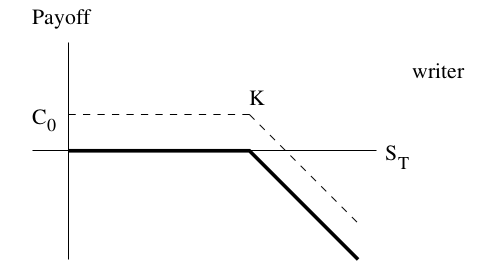
\includegraphics[width=1\linewidth]{Writer_call}
	\centering
	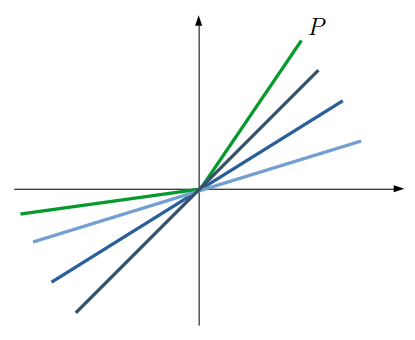
\includegraphics[width=0.6\linewidth]{H-B_2}
	\caption{Ejemplos de funcionales aportados por el teorema de Hahn-Banach.}
	\label{H-B-varios}
\end{figure} 

El teorema de Mazir-Orlicz-König, fijado un subconjunto convexo $ D $ de $ \vecSpace $, nos da solo los funcionales lineales que minoran a $ P $ y que cumplen
\[
\inf_D L = \inf_D P.
\]
En la imagen \ref{M-O-K-fotos} se muestra un ejemplo del teorema.
\begin{figure}[h!]
	%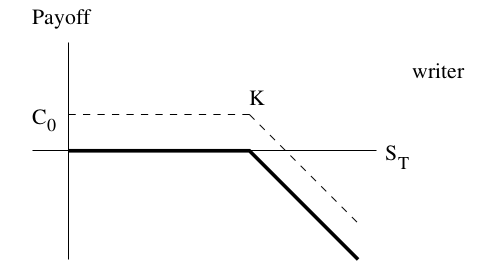
\includegraphics[width=1\linewidth]{Writer_call}
	\centering
	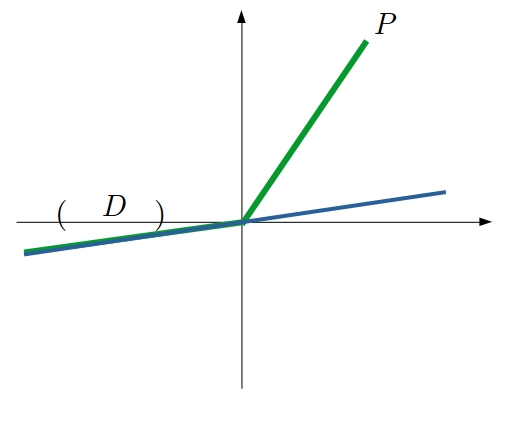
\includegraphics[width=0.6\linewidth]{M-O-K}
	\caption{Teorema de Mazur-Orlicz-König.}
	\label{M-O-K-fotos}
\end{figure} 

	\begin{proof}
		Sea $ \beta := \inf_D P $. En el caso de que $ \beta = -\infty $ por el teorema de Hanh-Banach tenemos que $ \exists L $ sobre \vecSpace tal que es lineal y $ L \leq P$. Así:
		\begin{center}
			$ L \leq P \Longrightarrow inf_D L \leq \inf_D P = -\infty \Longrightarrow inf_D L = \inf_D P.$ 
		\end{center}
		Supongamos entonces que $ \beta \in \RR $. Definimos el funcional auxiliar $ Q $ como en el lema \ref{lema2}. Del teorema de Hanh-Banach obtenemos que existe un funcional lineal $ L $ sobre \vecSpace tal que $ L \leq Q$ (como $ Q \leq P $ tenemos que $ L \leq P $). Sea $ d \in D $, entonces:
		\[
		L(d) = -L(-d) \geq -Q(-d) \geq \beta.
		\]
		Tomando ínfimo sobre $ d \in D $:
		\[
		\inf_D L \geq \beta = \inf_D P.
		\]
		Por otro lado, como $ L \geq P $:
		\[
		\inf_D L \leq\inf_D P.
		\]
		Juntando ambas desigualdades obtenemos $ \inf_D L =\inf_D P $.
	\end{proof}

\bigskip

%%% IGUALDAD
\newcommand{\normSpace}{E}
Antes de probar la eficiencia del teorema de Mazur-Orlicz-König en el siguiente apartado, presentamos una consecuencia bien conocida. En particular, nos será de utilidad posteriormente para el teorema de Separación. Recordemos dados $ \normSpace_1, \normSpace_2 $ dos espacios normados y $ T:\normSpace_1 \longrightarrow \normSpace_2 $ un operador lineal, entonces $ T $ es continuo si, y solo si, verifica la siguiente condición:
\[
\exists \alpha > 0 : \norm{T(x)} \leq \alpha \norm{x} \quad \forall x \in \normSpace_1,
\]
Consideramos el espacio vectorial dado por:
\[
\normSpace^* =  \lbrace T:\normSpace \longrightarrow \RR: T \text{ es lineal y continuo} \rbrace.
\]
conocido como el espacio dual (topológico) de $ E $. Para todo $ T \in \normSpace^* $ definimos su norma como:
\[
\norm{T} = \min \lbrace \alpha > 0:  \abs{T(x)} \leq \alpha \norm{x} \quad \forall x \in \normSpace\rbrace.
\]
De este modo, podemos escribir:
\begin{equation*}\label{desigNorma}
\abs{T(x)} \leq \norm{T} \norm{x}
\end{equation*}
siendo dicha desigualdad óptima. También podemos expresar su norma como el mínimo mayorante de un conjunto mayorado, es decir, el supremo:
\[
\norm{T} = \sup \lbrace \norm{T(x)}/\norm{x} : \forall x \in \normSpace \setminus \{0\}\rbrace.
\]
Para $  x \in \normSpace_1 \setminus \{0\} $ tenemos que $ \abs{T(x)}/\norm{x} = \norm{T(x/\norm{x})}$ y es claro que $ \{ x/\norm{x} : x \in \normSpace_1 \setminus \{0\}\} $ es la esfera unidad de $ \normSpace $ que notamos como $ S_\normSpace $. Si en vez de la esfera consideramos la bola unidad, $ B_\normSpace $ el supremo no varía. Efectivamente, si $ x \in B_\normSpace  $ se tiene que $ x = \norm{x}u $ con $ u \in  S_\normSpace$, y por ello $ \abs{T(x)} = \norm{x}\norm{T(u)} \leq \abs{T(u)} $ ya que $ \norm{x} \leq 1 $. De este modo, también tenemos que:
\begin{equation*}\label{normSup}
\norm{T} =\sup_{x \in B_\normSpace} \abs{T(x)}.
\end{equation*}

En este momento, estamos en disposición de enunciar y demostrar la igualdad que deseamos:

\bigskip
\begin{corolarioBox}\label{iguSupNor}
	Dado un espacio normado $ \normSpace $ y $ x \in \normSpace $, entonces se cumple que:
	\begin{equation}\label{iguNorm}
	\sup_{x^* \in B_{\normSpace ^ *}} x^*(x) = \norm{x}.
	\end{equation}
\end{corolarioBox}
\begin{proof}
	Sea $ x_0 \in E$ y sea $ D := \{x_0\} $. Consideramos el funcional 
	\begin{equation*}
	\begin{split}
	P:\normSpace \longrightarrow &\RR \\
	x \longmapsto &\norm{x}.
	\end{split}
	\end{equation*} 
	Es claro que $ P $ es sublineal y que $ D $ es convexo. Podemos aplicar el Teorema de Mazur-Orlicz-König, teorema \ref{M-O}, y obtenemos que existe un funcional $ L:\normSpace \longrightarrow \RR $ lineal tal que $ L \leq P $ e $ \inf_D L = \inf_D P $. Como $ L \leq P $, entonces 
	\begin{equation*}
	\norm{L(x)} \leq \norm{P(x)} = \norm{x} \quad \forall x \in \normSpace.
	\end{equation*}
	Concluimos que $ L $ es continua. Además, como tenemos que $ L \in \normSpace ^* $, llamamos $ L = x^* $ y llegamos a que $ \norm{L} = \norm{x^*}  \leq 1$, es decir, $ x^* \in  B_{\normSpace ^ *} $.  Por su parte, como  $ \inf_D L = \inf_D x^* = \inf_D P $ y $ D = \{x_0\} $ entonces, $ x^*(x_0) = \norm{x_0} $. De este modo, llegamos a que existe $ x^* \in B_{\normSpace^*} $ tal que $ x^*(x_0) = \norm{x_0} $. Si tomamos cualquier elemento $ y^* \in B_{\normSpace^*}  $, entonces \[ \norm{y^*(x_0)} \leq \norm{y^*} \norm{x_0} \leq \norm{x_0} \] y podemos asegurar que:
	\[
	\sup_{x^* \in B_{\normSpace ^ *}} x^*(x_0) = \norm{x_0}.
	\] 
	Como $ x_0 \in \normSpace $ es arbitrario, la desigualdad enunciada queda probada.
\end{proof}
\bigskip

\section{Teorema de la alternativa de Gordan. Reformulaciones.}
\newcommand{\ttt}{\textbf{\emph{t}}}
\newcommand{\sss}{\textbf{\emph{s}}}
\newcommand{\xx}{\textbf{\emph{x}}}
\newcommand{\yy}{\textbf{\emph{y}}}
\newcommand{\vv}{\textbf{\emph{v}}}
\newcommand{\ww}{\textbf{\emph{w}}}
\newcommand{\zz}{\textbf{\emph{z}}}

Una vez que disponemos de la herramienta fundamental, el teorema de Mazur-Orlicz-König, nos disponemos a dar una versión convexa del teorema de la alternativa de Gordan. Antes de ello, y haciendo uso de este teorema tipo Hahn-Banach, probaremos el lema de Simons, sobre cierta condición de optimalidad para funciones convexas. \\

Antes de comenzar, necesitamos hacer la siguiente definición. Para agilizar la lectura, cuando indicamos $ N\in \NN $ estamos suponiendo que $ N \geq 1 $. También, para $ N \in \NN $, notaremos con caracteres en negrita a los elementos de $ \RR^N $, por ejemplo, $  \ttt = (t_1,...,t_N)\in \RR^N$. 

\begin{definicion}
	Dado $ N \in \NN $ llamamos símplex unitario de $ \RR^N $ al conjunto de $ \RR^N $ definido como:
	\begin{equation*}
	\Delta_N := \left\lbrace \ttt \in \RR^N: \sum_{i=1}^{N}{t_i} = 1, \hspace{0.5em} t_1,...,t_N \geq 0 \right\rbrace .
	\end{equation*}
\end{definicion}

Recordamos ahora la noción de envolvente convexa de un subconjunto cualquiera $ X $ de un espacio vectorial $ \vecSpace $, que notamos como $ \mathrm{co}(X) $ y que se define como la intersección de todos los conjuntos convexos que contienen a $ X $. Nótese que $ \Delta_N = \mathrm{co}\{e_1,...e_N\} $. \\

Antes de continuar veamos que $ \Delta_N $ es convexo y compacto:

\begin{itemize}
	\item  Convexo: tenemos que comprobar que dados $ \ttt, \sss \in \Delta_N \text{ y } \lambda \in \lbrack 0,1 \rbrack $ entonces $ \lambda\ttt + (1-\lambda)\sss \in \Delta_N $. En efecto, las coordenadas $ \lambda t_i + (1-\lambda)s_i $ verifican:
	\begin{itemize}
		\item [i) ] $ \lambda t_i + (1-\lambda)s_i \geq 0 $ para todo $ i = 1,..., N $, ya que $ t_i, s_i \geq 0 $ y $ 0 \leq \lambda \leq 1 $.
		\item [ii) ] 
		\begin{equation*}
		\begin{split}
		\sum_{i=1}^{N} (\lambda t_i + (1-\lambda)s_i) &=   \lambda \sum_{i=1}^{N} t_i + (1-\lambda)\sum_{i=1}^{N} s_i \\
		&= \lambda + (1 - \lambda) \\ &= 1,
		\end{split}
		\end{equation*}ya que $ \sum_{i=1}^{N} t_i = \sum_{i=1}^{N} s_i = 1  $.
	\end{itemize}
	
	Por lo tanto, $ \lambda\ttt + (1-\lambda)\sss \in \Delta_N \text{ para todo }\lambda \in \lbrack 0,1 \rbrack $.
	
	\item Compacto: al encontrarnos en $ \RR^N $ y aplicando el conocido Teorema de Heine-Borel basta y sobra ver que $ \Delta_N $ es cerrado y acotado. Pero claramente es acotado por lo que nos centraremos en probar que es cerrado. Sea $ \lbrace \ttt_n \rbrace_{ n \in \NN} $ una sucesión de $ \Delta_N $ y sea $ \ttt_0 \in \RR^N $ tal que $ \lbrace \ttt_n \rbrace_{ n \in \NN} \longrightarrow \ttt_0 $. Tenemos que comprobar que $ \ttt_0 \in \Delta_N $. 
	\begin{itemize}
		\item[i) ] Como todas las coordenadas de cada $ \ttt_n $ para $ n \in \NN $ son no negativas las de $ \ttt_0 $ también lo son.
		\item[ii) ] La función $ f: \RR^N \longrightarrow \RR $ definida como $ f(\ttt) =  \sum_{i=1}^{N} t_i $ es continua. Claramente $ f(\ttt) = 1 $ para todo $ \ttt \in \Delta_N $ y por ello $ \lbrace f(\ttt_n) \rbrace_{ n \in \NN} \longrightarrow 1$. Por continuidad de $ f $ y unicidad de límite tenemos que $ f(\ttt_0) = 1 $ pero eso equivale a que la suma de sus componentes vale 1.
	\end{itemize} 
	
	Así, hemos demostrado que $ \ttt_0 \in \Delta_N $ y por lo tanto $ \Delta_N $ es compacto. 
\end{itemize}


\paragraph{}Antes de continuar, notamos que el espacio vectorial de todas las aplicaciones lineales de $ \RR^N $ a $ \RR $, con $ N \in \NN $, se puede identificar con $ \RR^N $. Esto se debe a que si $ L:\RR^N \longrightarrow \RR $ es lineal, entonces es de la forma $ L(\xx) = a_1x_1 + \cdots + a_Nx_N $, que se corresponde con $ \textbf{\emph{a}} = (a_1,\dots,a_N) \in \RR^N $. Del mismo modo, dado el vector tenemos la aplicación lineal asociada. En definitiva, el espacio dual de 
$ \RR^N $ se identifica con $ \RR^N $ .
\paragraph{} También presentamos el producto escalar usual en $ \RR^N $ que definimos como:
\[
\begin{split}
\langle \cdot, \cdot \rangle : \RR^N \times \RR^N \longrightarrow &\RR \\
(\xx, \yy) \longmapsto &\langle \xx, \yy \rangle = \sum_{i=0}^{N}x_iy_i.
\end{split}
\]

Antes de enunciar el lema de Simons, hacemos otra identificación, esta vez, correspondiente a un símplex unitario:
\bigskip
\begin{lemaBox}\label{lema2.1}
	Sea $ N \in \NN $ y $ S: \RR^N \longrightarrow \RR $ definida por: \[ S(\xx):=\max\{x_1,...,x_N\}.\] Entonces, $ S $ es sublineal. Además, si $ L:\RR^N \longrightarrow \RR $ es un funcional lineal tal que $ L \leq S $ entonces $ L $ es de la forma \[ L(\xx) = t_1 x_1 + ... + t_N x_N \] con $ (t_1,...,t_N) \in \Delta_N$. De hecho, el recíproco también es cierto, es decir, si $ L = \ttt = (t_1,...,t_N) \in \Delta_N $ entonces $ L \leq S $.
	
	%%%%%% NOTA %%%%%%%%
	%% Las aplicaciones lineales coninciden con el dual del espacio. Es decir, podemos identificar la aplicación con sus coeficientes obeniendo de ese modo un punto del espacio.
	
\end{lemaBox}
\begin{proof}
	Claramente, $ S $ es positivamente homogénea. También es sub\-aditiva ya que dados $ x,y \in \vecSpace $ : 
	\begin{equation*}
	\begin{split}
	S(\xx+\yy) &= \max \{x_1 + y_1, ..., x_N +y_N \}\\ 
	&\leq \max\{x_1, ..., x_N\} + \max \{y_1, ...,y_N\} = S(\xx) + S(\yy).
	\end{split}
	\end{equation*}
	
	Por ello, $ S $ es sublineal. Para terminar veamos que  \[\left\lbrace L:\RR^N \longrightarrow \RR : L \text{ lineal y }L\leq S \right\rbrace  =  \Delta_N \]
	a través de la correspondencia mostrada anteriormente entre $ \RR^N $ y su dual.
	
	\begin{itemize}
		\item[$ \supseteq $ )] Sea $ \mathbf{t} \in \Delta_N$, definimos $ L:\RR^N \longrightarrow \RR $ como $ L(\xx):= \langle \mathbf{t},\xx \rangle $. Es evidente que $ L $ es lineal en $ \xx $ al ser el producto escalar bilineal. Dado $ \xx \in \RR^N $,
		\begin{equation*}
		L(\xx) = \sum_{i=1}^{N}{t_i x_i} \leq \sum_{i=1}^{N}{t_i S(\xx)} = S(\xx)\sum_{i=1}^{N}{t_i} = S(\xx),
		\end{equation*}
		donde la primera desigualdad se debe a que $ x_i \leq S(\xx)$ para todo $ x_i$ con $ i=1,...,N $ y a que $ t_i \geq 0 $ ya que $ \mathbf{t} \in \Delta_N$. Esto también justifica la última igualdad ya que $ \sum_{i=1}^{N}{t_i} = 1 $.
		
		\item[$ \subseteq $ )] Sea $ L = \ttt = (t_1,...,t_N) \in \RR^N $ lineal tal que para todo $ \xx \in \RR^N $ cumple que $ \sum_{i=1}^{N}{t_i x_i} \leq S(\xx)$. Así, si tomamos $ e_i \in \RR^N $ donde $ e_i $ representa el i-ésimo elemento de la base usual de $ \RR^N $ con $ i=1,...,N $, entonces 		
		\begin{equation*}
		L(-e_i) = -t_i \leq 0 \Longrightarrow t_i \geq 0 \quad \forall i=1,...,N.
		\end{equation*}
		Si ahora llamamos $ e = \sum_{i=1}^{N}{e_i} $, obtenemos:
		\begin{equation*}
		\begin{rcases*}
		L(e) = \sum_{i=1}^{N}{t_i} \leq \max \{1, ...,1\} = 1 \\
		L(-e) = -\sum_{i=1}^{N}{t_i} \leq \max \{-1, ...,-1\} = -1
		\end{rcases*} \Longrightarrow \sum_{i=1}^{N}{t_i} = 1.
		\end{equation*}
		Concluimos entonces que $ L = \ttt = (t_1,...,t_N) \in \Delta_N $.
	\end{itemize}
	
\end{proof}
\bigskip

Enunciamos ahora el lema de Simons \cite{Simons2008}. Tal y como se ha mencionado antes, se trata de un resultado sobre funciones convexas y cierta condición de optimalidad: dos funciones distintas poseen el mismo ínfimo en un convexo. Esto sugiere el uso del teorema de Mazur-Orlicz-König.
\bigskip
\begin{lemaBox}[Simons]\label{Simons}
	Sea $ C $ un subconjunto convexo de un espacio vectorial y $ N \in \NN $. Dadas $  $ $ f_1, \dots, f_N : C \longrightarrow \RR $, funciones convexas, entones existe $ \ttt \in \Delta_N $ que cumple
	\[
	\inf_{c \in C}\left[ \max_{i=1\dots,N } f_i(c)\right] = \inf_{c \in C} \left[ \sum_{i=1}^{N} t_i f_i(c) \right].
	\] 
\end{lemaBox}
\begin{proof}
	Sea  $ \vecSpace = \RR^N $. Definimos $S:\vecSpace \longrightarrow \RR $ como \[ S(x_1, ..., x_N) := \max \{x_1, ..., x_N\}. \] Por el lema \ref{lema2.1}, $ S $ es sublineal. Tomamos el subconjunto:
	\[ 
	D = \{ (x_1, ..., x_N)\in V: \exists c \in C \quad \text{ tal que } \quad \forall i = 1,...N,\quad f_i(c) \leq x_i \}.
	\]
	Comprobemos en primer lugar que $ D $ es un subconjunto convexo de $ \vecSpace $. Sean $ x, y \in D $, por ello, existen $ c_x, c_y \in C $ tales que $ f_i (c_x) \leq x_i  $ y $ f_i (c_y) \leq y_i \quad \forall i=1,...,N $. Dado $ \lambda \in [0,1] $, llamamos $ c := (1-\lambda)c_x + \lambda c_y $ que pertenece a $ C $ por ser este convexo. Veamos que $ c $ es el elemento necesario de $ C $ para que cualquier combinación convexa de $ x $ e $ y $ esté en $ D $. Así, para todo $ i =1,...,N  $:	
	\[
	f_i(c) = f_i((1-\lambda)c_x + \lambda c_y) \leq (1-\lambda)f(c_x) + \lambda f(c_y) \leq (1-\lambda)x_i + \lambda y_i ,
	\]
	donde la primera desigualdad se debe a que las $ f_i $ son convexas y la segunda a que $ x,y \in D $. Por ello, $ (1-\lambda)x_i + \lambda y_i \in D , \quad \forall \lambda \in [0,1] $ por lo que $ D $ es convexo. Aplicando el Teorema de Mazur-Orlizc-König, existe $ L $ funcional lineal en $ \vecSpace $ tal que $ L \leq S $ e $ \inf_D L = \inf_D S $. \\
	
	Nuevamente, por el lema \ref{lema2.1} tenemos que $ L = \ttt \in \Delta_N$. Finalmente:
	\[
	\inf_D L =\inf_{c \in C} \left[ \sum_{i=1}^{N} t_i f_i(c) \right]
	\]
	e
	\[
	\inf_D S = \inf_{c \in C}\left[ \max_{i=1\dots,N } f_i(c)\right]
	\]
	por lo que 
	\[ \inf_{c \in C}\left[ \max_{i=1\dots,N } f_i(c)\right] = \inf_{c \in C} \left[ \sum_{i=1}^{N} t_i f_i(c) \right]. \] 
\end{proof}
\bigskip
Enuciamos ahora el Teorema de la Alternativa de Gordan en su versión clásica.
\bigskip
\begin{teoremaBox}[Teorema de la alternativa de Gordan]\label{GordanClasic}
	Dados $N, M \in \NN   $, sean $ \{\xx_1,...\xx_N\}$ con $ \xx_i \in \RR^M \text{ para } i=1,...,N$. Entonces una, y solo una, de la siguientes afirmaciones se cumple:
	
	\begin{itemize}
		\item[i*)] $ \exists \mathbf{t} \in \Delta_N $ tal que  $  0 = \displaystyle \sum_{i=1}^{N}{t_i \xx_i}$.
		\item[ii*)] $ \exists \yy \in \RR^M $ tal que cumple $ \displaystyle \max_{i=1,...,N} \langle \yy, \xx_i \rangle < 0 $.
	\end{itemize}
\end{teoremaBox}
\bigskip
Omitimos esta demostración ya que a continuación mostramos la versión convexa del mismo y será la que probaremos. Después veremos que la versión convexa  implica la clásica por lo que quedará probada. Antes de continuar, destacar que la interpretación geométrica de este resultado se observa en la imágen \ref{fig:gordan-clasic}.

\begin{figure}[h!]
	\begin{minipage}{0.5\textwidth}
		\centering
		%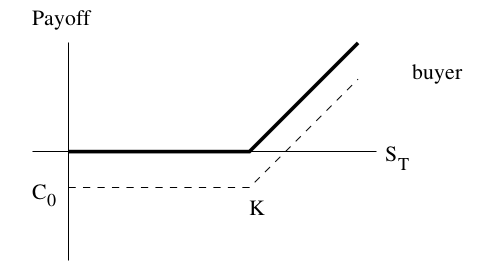
\includegraphics[width=1\linewidth]{Buyer_call} 
		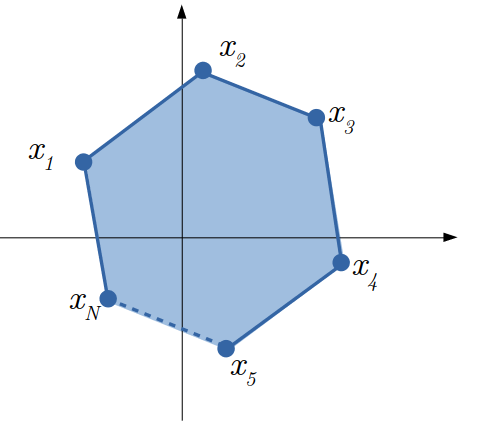
\includegraphics[width=1\linewidth]{Gordan-i*} 
		%\caption{Alternativa $ i*) $.}
		%\label{fig:gordan-i*}
	\end{minipage}
	\begin{minipage}{0.5\textwidth}
		%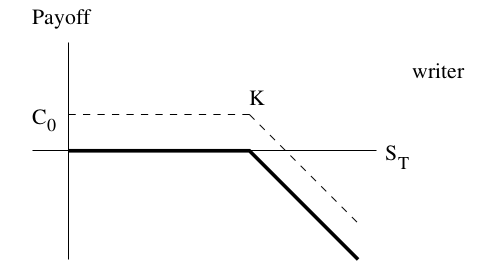
\includegraphics[width=1\linewidth]{Writer_call}
		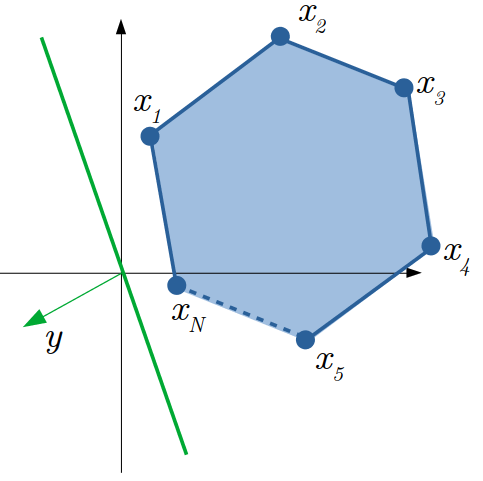
\includegraphics[width=1\linewidth]{Gordan-ii*}
		%\caption{Alternativa $ ii*) $.}
		%\label{fig:gordan-ii*}
	\end{minipage}
	\caption{A la izquierda alternativa $ i*) $ y a la derecha la alternativa $ ii*) $.}
	\label{fig:gordan-clasic}
\end{figure}

\bigskip
\begin{teoremaBox}[Teorema de la Alternativa de Gordan-versión convexa]\label{Gordan}
	Sean $ C $ un subconjunto convexo de un espacio vectorial, $ N \in \NN $ y  $ f_1,...,f_N : C \longrightarrow \RR $ funciones convexas. Entonces una, y solo una, de la siguientes afirmaciones se cumple:
	\begin{itemize}
		\item[i)] $ \exists \mathbf{t} \in \Delta_N $ tal que $ 0 \leq \displaystyle \inf_{c\in C}  \sum_{i=1}^{N}{t_i f_i (c)}$.
		\item[ii)] $ \exists c \in C $ que cumple $\displaystyle \max_{i=1\dots,N } f_i(c) < 0 $.
	\end{itemize}
\end{teoremaBox}
\begin{proof}
	Veamos que las alternativas $ i)$ y $ ii) $ son excluyentes y exhaustivas. Para ello, veamos que $ \neg i) \Longleftrightarrow ii) $. Suponemos inicialmente que $  \inf_{ c\in C}\left[\max_{i=1\dots,N } f_i(c) \right] \in \RR $.
	
	\begin{itemize}
		\item [$ \Leftarrow $)] Si existe $ c_0 \in C $ tal que $ \max_{i=1\dots,N } f_i(c) < 0 $, entonces, dado $ \ttt \in \Delta_N $,
		\[
		\inf_{ c \in C} \sum_{i=0}^{N}t_i f_i(c) \leq \sum_{i=0}^{N}t_i f_i(c_0) < 0
		\]
		donde la última desigualdad se debe a que $ \ttt \in \Delta_N $. Hemos probado entonces $ \neg i) $.
		\item[$ \Rightarrow $)] 	Si aplicamos el lema de Simons, lema \ref{Simons}, a las funciones $ f_1,...,f_N $ obtenemos:
		
		\begin{equation*}
		\exists t \in \Delta_N \text{ : } \inf_{ c\in C}\left[\max_{i=1\dots,N } f_i(c) \right] = \inf_{c \in C} \sum_{i=1}^{N}t_i f_i (c).
		\end{equation*}
		Entonces, de $ \neg i) $ sabemos que, para este $ \ttt \in \Delta_N $ (como para cualquier otro)
		\[
		\inf_{ c \in C} \sum_{i=0}^{N}t_i f_i(c) < 0
		\]
		luego
		\[
		\inf_{ c\in C}\left[\max_{i=1\dots,N } f_i(c) \right] < 0,
		\]
		como queríamos demostrar.
		
	\end{itemize}
	
	Para finalizar, si $  \inf_{ c\in C}\left[\max_{i=1\dots,N } f_i(c) \right] =-\infty $ es claro que estamos en el caso $ ii) $ y se prueba como en el caso de que dicho ínfimo sea un valor real.
\end{proof}
\bigskip
Destacamos las siguientes observaciones:
\bigskip
\begin{observacion}
	Esta versión convexa del teorema implica la versión clásica del mismo.
\end{observacion}

Para ello, basta aplicar la versión convexa del teorema a $ C := \RR^M $ y a las funciones $ f_1,...,f_N : C \longrightarrow \RR $ definidas por \[ f_i(c):=\langle c, \xx_i \rangle , \forall i=1,...,N.\] Notar que las funciones $ f_1,...,f_N $ son lineales por la izquierda y como consecuencia son convexas. En este caso, la alternativa $ ii) $ implica $ ii*) $ ya que:

\begin{equation*}
\exists c \in C = \RR^M \text{ : } \max_{i=1,...,N} {\langle c,x_i \rangle}  =  \max_{i=1,...,N}f_i (c) < 0 .
\end{equation*}
Por su parte, la alternativa $ i) $ nos da:
\begin{equation*}
\exists \mathbf{t} \in \Delta_N \text{ : } 0 \leq \inf_{c \in \RR^M}  \sum_{i=1}^{N}{t_i f_i(c) } = \inf_{c \in \RR^M} \sum_{i=1}^{N}{t_i\langle c, \xx_i \rangle} = \inf_{c \in \RR^M} \langle c, \sum_{i=1}^{N}{t_i 	\xx_i} \rangle. 
\end{equation*}
Hemos obtenido por ello que  $0  \leq \inf_{c \in \RR^M} \langle c, \sum_{i=1}^{N}{t_i \xx_i} \rangle  $ lo que significa que $ 0 \leq \langle c, \sum_{i=1}^{N}{t_i \xx_i} \rangle  $ para todo $ c \in \RR^M $. Usando la bilinealidad del producto escalar:
\[
0 \leq \langle -c, \sum_{i=1}^{N}{t_i \xx_i} \rangle \Longleftrightarrow 	0 \leq -\langle c, \sum_{i=1}^{N}{t_i \xx_i} \rangle 
\Longleftrightarrow  \langle c, \sum_{i=1}^{N}{t_i \xx_i}\rangle \leq 0, \quad \forall c \in \RR^M.
\]
Juntando ambas desigualdades obtenemos que $ 0 =  \langle c, \sum_{i=1}^{N}{t_i \xx_i}\rangle, \quad \forall c \in \RR^M $. Como la igualdad anterior se cumple para todo elemento de $ \RR^M $ entonces podemos deducir que $ \sum_{i=1}^{N}{t_i \xx_i} = 0 $	ya que $ \sum_{i=1}^{N}{t_i \xx_i} \in (\RR^M)^{\perp} = \{0\} $. Así pues, tenemos que $ i) $ equivale a $ i*) $. \hspace{5.7cm}\qedsymbol 

\bigskip
\begin{observacion}
	El lema de Simons (lema \ref{Simons}) y el teorema convexo de la Alternativa de Gordan (teorema \ref{Gordan}) son equivalentes.
\end{observacion}

\paragraph{} Ya hemos visto que el Lema de Simons implica el Teorema de la Alternativa de Gordan. Veamos que el recíproco también es cierto.  \\

Llamamos $ \alpha := \inf_{ c\in C}\left[\max_{i=1\dots,N } \{f_i(c)\} \right] $. Si $ \alpha = -\infty $. Por el lema \ref{lema2.1} sabemos que $ \forall \ttt \in \Delta_N $ se cumple que $ \sum_{i=1}^{N} t_i f_i(c) \leq \max_{i=1\dots,N } \{f_i(c)\}$ para todo $ c \in C$. Tomando ínfimos en C:
\[
\inf_{c \in C}\left[ \sum_{i=1}^{N} t_i f_i(c) \right] \leq \inf_{ c\in C}\left[\max_{i=1\dots,N } \{f_i(c)\} \right] = -\infty \Longrightarrow \inf_{ c \in C}\left[ \sum_{i=1}^{N} t_i f_i (c)\right] = -\infty 
\]
y por ello $ \forall \ttt \in \Delta_N $ (en particular para uno cualquiera) se cumple que

\[
\inf_{c \in C}\left[ \sum_{i=1}^{N} t_i f_i (c) \right] = \inf_{ c\in C}\left[\max_{i=1\dots,N } \{f_i(c)\} \right]. \]
Supongamos ahora que $ \alpha \in \RR $. Sean las funciones $ g_1, ..., g_N: C \longrightarrow \RR $ definidas como $ g_i = f_i - \alpha $ con $ i=1,...,N$. Veamos que las funciones $ g_1, ..., g_N $ son convexas como consecuencia de que $ f_1, ..., f_N $ lo son. Sean $ i = 1, \dots, N $, $ c_1,c_2 \in C $ y $ \lambda \in \left[0,1\right] $:
\begin{equation*}
\begin{split}
g_i(\lambda c_1 + (1-\lambda) c_2) &= f_i(\lambda c_1 + (1-\lambda) c_2) - \alpha \\
&\leq \lambda f_i(c_1) + (1-\lambda)f_i(c_2) - \alpha \\
&= \lambda f_i(c_1) + (1-\lambda)f_i(c_2) - \lambda \alpha + (1-\lambda)\alpha \\
&= \lambda( f_i(c_1) - \alpha ) + (1-\lambda) (f_i (c_2) - \alpha) \\
&= \lambda g_i(c_1) + (1-\lambda) g_i (c_2).
\end{split}
\end{equation*}
Obtenemos así que $ g_i $ es convexa para todo $ i = 1, ..., N $. Si usamos el Teorema de la Alternativa de Gordan obtenemos que solo se puede dar una y solo de las siguientes posibilidades:

\begin{itemize}
	\item[i)] $ \exists \mathbf{t} \in \Delta_N $ tal que $ 0 \leq \inf_{c \in C}  \sum_{i=1}^{N}{t_i g_i (c)}$.
	\item[ii)] $ \exists c \in C $ que cumple $ \max_{i=1\dots,N } \{g_i(c)\}  < 0 $.
\end{itemize}

Razonemos que no se puede dar $ ii) $. Si fuese así, tendríamos que $ \exists c \in C $ tal que $ \max_{i=1\dots,N } \{g_i(c)\} =  \max_{i=1\dots,N } \{f_i(c) - \alpha \} < 0 $. En particular, se cumpliría \[ f_j(c) - \alpha < 0 \Longrightarrow f_j(c) < \alpha = \inf_{ c\in C}\left[\max_{i=1\dots,N } \{f_i(c)\} \right],\hspace{2mm} \forall  j \in {1,...,N}. \] Esto es imposible por la propia definición de $ \alpha $. Por ello, afirmamos que $ \exists \mathbf{t} \in \Delta_N $ tal que $ 0 \leq \inf_{C}  \sum_{i=1}^{N}{t_i g_i}$. Desarrollando el sumatorio:
\begin{equation*}
\begin{split}
0 &\leq \inf_{c \in C}  \sum_{i=1}^{N}{t_i g_i (c)}\\
 &= \inf_{c \in C}  \sum_{i=1}^{N}{t_i(f_i(c) - \alpha)} \\
&= \inf_{c \in C} \left[ \sum_{i=1}^{N}{t_i f_i(c)} - \sum_{i=1}^{N}{t_i\alpha} \right]\\
&= \inf_{c \in C} \left[ \sum_{i=1}^{N}{t_i f_i(c)} -\alpha \sum_{i=1}^{N}{t_i} \right] \\ 
&= \inf_{c \in C} \left[ \sum_{i=1}^{N}{t_i f_i(c)} - \alpha \right] \\
&= \inf_{c \in C} \left[ \sum_{i=1}^{N}{t_i f_i(c)}\right] - \alpha.
\end{split}
\end{equation*}
Por lo tanto:
\[
0 \leq \inf_{c \in C} \left[ \sum_{i=1}^{N}{t_i f_i(c)}\right] - \alpha \Longleftrightarrow \inf_{c \in C}\left[ \max_{i=1\dots,N } \{f_i(c)\}\right] = \alpha  \leq \inf_{c \in C} \left[ \sum_{i=1}^{N}{t_i f_i(c)}\right].
\]
El lema \ref{lema2.1} nos aporta la otra desigualdad y llegamos nuevamente a que $ \exists \ttt \in \Delta_N $ que cumple:
\[
\inf_{c \in C}\left[ \max_{i=1\dots,N } \{f_i(c)\}\right] = \inf_{c \in C} \left[ \sum_{i=1}^{N}{t_i f_i(c)}\right]. \]
\hspace{12.2cm}\qedsymbol 

\bigskip

Mencionemos antes de terminar que el teorema de la alternativa de Gordan no solo es equivalente al lema de Simons. Otro tipo de teorema de la alternativa equivalente es el lema de Farkas que estudiaremos en el capítulo 3. Son muchos los teoremas de la alternativa que se conocen, y siempre vinculados a la optimización: véase, por ejemplo, la amplia muestra que aparece recogida en \cite{giorgi2004mathematics}. A modo de ejemplo, y usando la notación clásica matricial, enunciaremos algunos de los resultados más conocidos:

\bigskip
\begin{teoremaBox}[Motzkin]
Dados $ N,M \in \NN $, tomamos las matrices $ A,B,D \in \RR^{M\times N} $. Entonces una, y solo una, de las siguientes condiciones se cumple:
\begin{itemize}
\item[m1)] $ \exists \xx \in \RR^N  $ tal que $ A\xx = 0 $, $ B\xx \geq 0 $ y $ D\xx > 0$.
\item[m2)] $ \exists \yy, \vv, \ww \in \RR^M $ tales que $ \yy^T A + \vv^T B + \ww^T D = 0 $, $ \vv \geq 0 $ y $\ww \geq 0 $.
\end{itemize} 
\end{teoremaBox}
\bigskip

\begin{teoremaBox}[Tucker]
Dados $ N,M \in \NN $, tomamos $ A,B,D \in \RR^{M\times N} $. Entonces una, y solo una, de las siguientes condiciones se cumple:
	\begin{itemize}
		\item[m1)] $ \exists \xx \in \RR^N  $ tal que $ A\xx = 0 $, $ B\xx \geq 0 $ y $ D\xx \geq 0$.
		\item[m2)] $ \exists \yy, \vv, \ww \in \RR^M $ tales que $ \yy^T A + \vv^T B + \ww^T D = 0 $, $ \vv \geq 0 $ y $\ww > 0 $.
	\end{itemize} 
\end{teoremaBox}
\bigskip

\begin{teoremaBox}[Primer teorema de la alternativa de Fenchel]
	Dados $ N,M \in \NN $, tomamos $ A,B \in \RR^{M\times N} $. Entonces una, y solo una, de las siguientes condiciones se cumple:
	\begin{itemize}
		\item[m1)] $ \exists \xx, \zz \in \RR^N  $ tales que $ A\xx + B\zz = 0 $, $ \xx \geq 0 $ y $ \zz \geq 0$.
		\item[m2)] $ \exists \yy \in \RR^M $ tal que $ \yy^T A \geq 0 $ e $ \yy^T B > 0 $.
	\end{itemize} 
\end{teoremaBox}
\bigskip

\chapter{Alternativa y minimax}
\newcommand{\topSpace}{X}
\newcommand{\topSpaceY}{Y}
Este capítulo se centra en el uso de los teoremas de la alternativa en la teoría minimax, surgida a finales de la década de 1920 de la mano de J. von Neumann en el seno de la teoría de juegos. Sin embargo, nosotros aplicaremos un teorema minimax deducido del teorema de la alternativa de Gordan para obtener resultados de separación de convexos
\section{Una desigualdad minimax}
\paragraph{}En esta sección llegaremos a otro de los resultados clave del trabajo. Será uno de los denominados teoremas minimax. A rasgos generales y a modo introductorio, podemos decir que un teroema minimax es un resultado que afirma, bajo ciertas hipótesis, que:
\[
\inf_{y \in Y} \sup_{x \in X} f(x,y) = \sup_{x \in X} \inf_{y \in Y} f(x,y),
\] 
donde $ X \text{ e } Y$ son conjuntos y $ f: X \times Y \longrightarrow \RR $. Obviamente, esta igualdad no es cierta en general tal y como mostramos en el siguiente ejemplo. Definimos $ f:\{0,1\} \times \{0,1\} \longrightarrow \RR$ como:
\[
f(x,y) = \begin{cases}
0, & \mbox{si $ x=y $ } \\
1, & \mbox{si $ x\neq y$ }
\end{cases}.
\]
Por un lado tenemos
\[
\inf_{ y \in Y}\sup_{x \in X} f(x,y) = \min_{ y \in Y}\max_{x \in X} f(x,y) = \min_{ y \in Y}\{1\} = 1,
\]
y por otro
\[
\sup_{x \in X} \inf_{ y \in Y}f(x,y) = \max_{x \in X}\min_{ y \in Y}f(x,y) = \min_{ y \in Y}\{0\} = 0.
\]
Notemos que la desigualdad 
\[
\inf_{y \in Y} \sup_{x \in X} f(x,y) \geq \sup_{x \in X} \inf_{y \in Y} f(x,y)
\] 
siempre se da ya que si $ (x_0, y_0) \in X \times Y $, entonces:
\[
\sup_{x \in X} f(x,y_0) \geq f(x_0,y_0) \geq \inf_{y \in Y}f(x_0,y) .
\]
Por ello, los teoremas minimax solo nos aportan la otra desigualdad necesaria, de ahí que este tipo de resultados se conozcan también como desigualdad minimax. \\

Antes de continuar, exponemos la siguiente definición que aparecerá posteriormente en el teorema. Se trata de una propiedad más débil que la continuidad para funciones reales. 
\bigskip
\begin{definicion}
Sea $ \topSpace $ un espacio topológico. Decimos que $ f:\topSpace \longrightarrow \RR $ es superiormente semicontinua en $ X $ si para todo $ r \in \RR $ se cumple que el conjunto $ \lbrace x \in \topSpace : f(x) \geq r \rbrace $ es cerrado.
\end{definicion}
\bigskip
Es claro que toda función continua en $ \topSpace $ es superiormente semicontinua, aunque el recíproco no es cierto, tal y como prueba la función $ f:\RR \longrightarrow \RR $ dada por 
\[
f(x) = \begin{cases}
0, & \mbox{si $ x < 0 $ } \\
1, & \mbox{si $x \geq 0$ }.
\end{cases}
\]

Para funciones superiormente semicontinuas, podemos enunciar los siguientes resultados. En particular, el lema \ref{supConMax} es análogo al del caso continuo.
\bigskip
\begin{lemaBox}\label{infDeSupSemi}
El ínfimo de una familia de funciones reales $ (f_\lambda)_{\lambda \in \Lambda} $ definidas en el mismo espacio topológico $ X $, si es finito, determina una función superiormente semicontinua. 
\end{lemaBox}
\bigskip

Este hecho es inmediato de la definición pues dado $ r \in \RR $, 
\begin{equation*}
\begin{split}
	\{ x \in X: \hspace{1.5mm} \inf_{ \lambda \in \Lambda}f_\lambda(x) \geq r\} &= \{ x \in X: \hspace{1.5mm} \lambda \in \Lambda \Longrightarrow f_\lambda(x) \geq r\}\\
	&=\bigcap_{\lambda \in \Lambda} \{ x \in X: \hspace{1.5mm}f_\lambda(x) \geq r \},
\end{split}
\end{equation*}
que es cerrado por ser intersección de cerrados. \\

\bigskip
\begin{lemaBox}\label{supConMax}
Si $ X $ es un espacio topológico compacto y $ f:X \longrightarrow \RR $ es superiormente semicontinua, entonces $ f $ alcanza su supremo en $ X $.
\end{lemaBox}
\bigskip

La demostración de este resultado está recogida en \cite{borwein}. \\

En estos momentos nos encontramos en condiciones de enunciar y demostrar el siguiente teorema minimax, más general que el de von Neumann. Los ingredientes de la prueba son las condiciones topológicas que se suponen y el teorema de de la alternativa de Gordan, versión convexa, en forma equivalente del lema de Simons. Seguimos la demostración dada por \cite{Simons2008}.
\bigskip
\begin{teoremaBox}\label{MinMax}
Sean $ \topSpace,\hspace{0.5mm} \topSpaceY $ subconjuntos convexos de sendos espacios vectoriales (no tienen que ser el mismo) tal que $ \topSpace $ está dotado de una topología que lo hace compacto. Supongamos además que $ f:  \topSpace \times \topSpaceY \longrightarrow \RR $ es:
\begin{itemize}	
\item[i)] cóncava y superiormente semicontinua en $ \topSpace $ y
\item[ii)] convexa en $ \topSpaceY $.
\end{itemize}
Entonces:
\begin{equation*}\label{eqMinMax}
\inf_{y \in Y} \max_{x \in X} f(x,y) = \max_{x \in X} \inf_{y \in Y} f(x,y).
\end{equation*}
\end{teoremaBox}
\begin{proof}
En primer lugar, por lemas \ref{infDeSupSemi} y \ref{supConMax}  podemos escribir máximo en ambos casos en vez de supremo ya que $ f $ es superiormente semicontinua en $ \topSpace $, por ello $ \inf_{y \in Y} f(x,y) $ también lo es y $ \topSpace $ es compacto. Como hemos explicado anteriormente, solo necesitamos la desigualdad 
\begin{equation}\label{desAux1}
\inf_{y \in Y} \max_{x \in X} f(x,y) \leq \max_{x \in X} \inf_{y \in Y} f(x,y).
\end{equation}  Definimos $ \alpha := \inf_{y \in Y} \max_{x \in X} f(x,y) $. Si $ \alpha = -\infty $ no hay nada que probar, por lo que supondremos que $ \alpha \in \RR $. Primero vamos a reescribir el resultado a probar. La desigualdad (\ref{desAux1}) es equivalente a
\[
\exists x_0 \in X:\text{ }\alpha \leq \inf_{y \in Y} f(x_0,y),
\]
ya que si existe un elemento en $ X $ que lo cumpla el máximo también lo cumplirá y recíprocamente. O lo que es lo mismo:
\[
\exists x_0 \in X:\text{ }y \in \topSpaceY \Longrightarrow \alpha \leq f(x_0,y),
\]
o lo que es igual, 
%ya que al menos x_0 está en dicho intersección
\begin{equation}\label{desAux2}
\bigcap_{y\in \topSpaceY}\{x \in \topSpace: \alpha \leq f(x, y) \} \neq \emptyset.
\end{equation}
Como $ f $ es superiormente semicontinua en $ \topSpace $ estamos ante una intersección de cerrados. Usando la propiedad de intersección finita ($ \topSpace $ es compacto) obtenemos que \eqref{desAux2} equivale a
\[
N\in\NN, \text{ }y_1,\dots,y_N \in \topSpaceY \Longrightarrow \bigcap_{i=1}^{N}\{x \in \topSpace: \alpha \leq f(x, y_i) \} \neq \emptyset.
\]
\[
\big\Updownarrow
\]
\[
N\in\NN, \text{ }y_1,\dots,y_N \in \topSpaceY \Longrightarrow \exists x_0\in\topSpace:\alpha \leq \min_{i=1\dots,N }f(x_0,y_i).
\]
\[
\big\Updownarrow
\]
\begin{equation}\label{desAux}
N\in\NN, \text{ }y_1,\dots,y_N \in \topSpaceY \Longrightarrow \alpha \leq \max_{x \in X} \min_{i=1\dots,N }f(x,y_i).
\end{equation}
Esta última condición es cierta. En efecto, sean $ N \in \NN $ e \vecN{y}$ \in \topSpaceY$. Aplicamos el lema de Simons, lema \ref{Simons}, tomando $ C := \topSpace $ y $ f_i: \topSpace \longrightarrow \RR $ definidas como \[
 f_i(x):=-f(x,y_i), \quad i=1,\dots,N.\]
Como $ f $ es cóncava respecto a $ X $ tenemos que las $ f_i $ son convexas en $ X $ con $  i=1,\dots,N $. De este modo, existe $ \ttt \in \Delta_N$ tal que
\[
\inf_{x \in \topSpace} \max_{i=1\dots,N } \{f_i(x)\} = \inf_{x \in \topSpace} \left[ \sum_{i=1}^{N} t_i f_i(x) \right].
\] 
Si ponemos la igualdad en función de $ f $ y recordamos que alcanza el supremo en $ X $,
\[
\inf_{x \in \topSpace} \max_{i=1\dots,N } \{-f(x,y_i)\} = \inf_{x \in \topSpace} \left[ \sum_{i=1}^{N} t_i (-f(x,y_i)) \right]
\] 
\[
\big\Downarrow
\]
\[
\max_{x \in \topSpace} \min_{i=1\dots,N } \{f(x,y_i)\} = \max_{x \in \topSpace} \left[ \sum_{i=1}^{N} t_i f(x,y_i) \right]. 
\] 
Al ser $ f $ convexa en $ \topSpaceY $:
\begin{equation*}
\begin{split}
\max_{x \in \topSpace} \min_{i=1\dots,N } \{f(x,y_i)\} &= \max_{x \in \topSpace} \left[ \sum_{1=1}^{N} t_i f(x, y_i) \right] \\
&\geq \max_{x \in \topSpace} \left[ f(x,\sum_{i=1}^{N} t_i y_i) \right] \\
&\geq \inf_{y \in Y} \max_{x \in \topSpace} f(x,y) \\
&= \alpha.
\end{split}
\end{equation*}
Hemos probado entonces la desigualdad (\ref{desAux}) y con ello el teorema.
\end{proof}
\bigskip
\input{capitulos/separación.tex}

\chapter{Optimización}
Si en el capítulo anterior dábamos las primeras aplicaciones del teorema de Gordan en forma de teorema minimax y, consecuentemente, de teoremas de separación, ahora usamos los teoremas de la alternativa en su contexto original: a optimización. Tras presentar un nuevo resultado de la alternativa, el lema de Farkas, abordamos el estudio de dos problemas clásicos: uno de dualidad en programación lineal; otro de paso de un problema de optimización con restricciones (en este caso de tipo desigualdad) a otro sin restricciones, vía los teoremas de Fritz-John y Karush-Kuhn-Tucker. Para el primero de ellos usamos el de Farkas y para el segundo el teorema de Gordan en su versión clásica.

\section{Lema de Farkas}
\newcommand{\bb}{\textbf{\emph{b}}}
\newcommand{\cc}{\textbf{\emph{c}}}

En el capítulo anterior hemos vimos como uno de los teoremas de separación implica el único teorema de la alternativa que hemos visto hasta el momento. Ahora, vamos a deducir de manera parecida otro teorema de la alternativa. Antes exponemos la siguiente definición.

\begin{definicion}
	Dados $ M, N \in \NN $ y $ \{\xx_1,\dots, \xx_M \} \subset \RR^N  $, llamamos cono generado por $ \{\xx_1,\dots, \xx_M \} $ al conjunto de $ \RR^N $ dado por:
	\begin{equation*}
	\mathrm{cone}\{\xx_1,\dots, \xx_M \} := \left\lbrace \sum_{j=1}^{N}{\mu_j \xx_j } : \text{ } \mu_1,...,\mu_N \geq 0 \right\rbrace .
	\end{equation*}
\end{definicion}

Veamos que $ \mathrm{cone}\{\xx_1,\dots, \xx_M \} $ es un subconjunto convexo y cerrado de $ \RR^N $:

\begin{itemize}
	\item  Convexo: tenemos que comprobar que dados $ \ttt, \sss \in \mathrm{cone}\{\xx_1,\dots, \xx_M \} $ y $ \lambda \in \lbrack 0,1 \rbrack $ entonces $ \lambda\ttt + (1-\lambda)\sss \in \mathrm{cone}\{\xx_1,\dots, \xx_M \} $. En efecto:
	
	\begin{equation*}
	\begin{split}
	\lambda\ttt + (1-\lambda)\sss &=   \lambda \sum_{j=1}^{N}{\mu_j^t \xx_j } + (1-\lambda)\sum_{j=1}^{N}{\mu_j^s \xx_j } \\
	&= \sum_{j=1}^{N}{\lbrack \lambda \mu_j^t \xx_j  + (1-\lambda)\mu_j^s\xx_j \rbrack} \\
	&= \sum_{j=1}^{N}{\lbrack \lambda \mu_j^t  + (1-\lambda)\mu_j^s \rbrack \xx_j}.
	\end{split}
	\end{equation*}
	Como $ \mu_j^t \text{ y } \mu_j^s $ son no negativos, entonces $ \lambda \mu_j^t  + (1-\lambda)\mu_j^s  $ también es una cantidad no negativa para $ j=1,\dots,M $. Así, podemos concluir que $ \lambda\ttt + (1-\lambda)\sss \in \mathrm{cone}\{\xx_1,\dots, \xx_M \} $ y por tanto es un subconjunto convexo.
	
	\item Cerrado: sea $ \lbrace \ttt_n \rbrace_{ n \in \NN} $ una sucesión de $ \mathrm{cone}\{\xx_1,\dots, \xx_M \} $ y sea $ \ttt_0 \in \RR^N $ tal que $ \lbrace \ttt_n \rbrace_{ n \in \NN} \longrightarrow \ttt_0 $. Si notamos $ \ttt_n = \sum_{j=1}^{N}{\mu_j^n \xx_j }$, entonces:
	\[
	\lbrace \ttt_n \rbrace_{ n \in \NN} = \lbrace \sum_{j=1}^{N}{\mu_j^n \xx_j } \rbrace_{ n \in \NN} \longrightarrow \sum_{j=1}^{N}{\mu_j^0 \xx_j } = \ttt_0.
	\]
	Como para cada $ \ttt_n $ cumple que $ \mu_j^n \geq 0$ con $ j=1,\dots,N $ podemos asegurar que $ \mu_j^0 \geq $ con $ j=1,\dots,N $. Hemos demostrado que $ \ttt_0 $ se expresa como combinación de $ \{\xx_1,\dots, \xx_M \} $ con coeficientes no negativos. Por lo tanto, $ \ttt_0 \in \mathrm{cone}\{\xx_1,\dots, \xx_M \}  $ y por consiguiente es cerrado. 
\end{itemize} 

Enunciamos ahora otro de los teoremas de la alternativa más conocidos.
\bigskip
\begin{lemaBox}[Farkas]
	Sean $ M,N \in \NN $ y $ \{\xx_1,\dots, \xx_M \} \subset \RR^N $ y $ \bb \in \RR^N $. Entonces una, y solo una, de la siguientes alternativas se cumple:
	\begin{itemize}
		\item[i')] $ \exists \mu_1,\dots,\mu_M \geq 0 $ tal que $ \bb = \sum_{j=1}^{M} \mu_j \xx_j$.
		\item[ii')]$ \exists \zz_0 \in \RR^N $ que cumple que:
		\begin{enumerate}
			\item $ \displaystyle\max_{ j=1,\dots,M} \langle \zz_0, \xx_j \rangle \leq 0$ y
			\item $ \langle \zz_0, \bb\rangle > 0$.
		\end{enumerate} 
	\end{itemize}
\end{lemaBox}

\begin{proof}
	Planteamos las siguientes alternativas, que obviamente son excluyentes, y que implican las de la tesis del lema:
	\begin{itemize}
		\item[a)] $\bb \in \mathrm{cone}\{\xx_1,\dots, \xx_M \} $. Estamos en el caso $ i') $  ya que:
		\[
		\bb \in \left\lbrace \sum_{j=1}^{N}{\mu_j \xx_j } : \text{ } \mu_1,...,\mu_N \geq 0 \right\rbrace .
		\]
		\item[b)] $ \bb \notin \mathrm{cone}\{\xx_1,\dots, \xx_M \} $. Por su parte, esta alternativa equivale a $ ii') $. En efecto: 
		
		\begin{itemize}
			\item[$ ii') \Longrightarrow b) $] Razonamos por reducción al absurdo. Suponemos por ello que el elemento $ \bb \in \mathrm{cone}\{\xx_1,\dots, \xx_M \} $, entonces, podemos expresar $ \bb =  \sum_{j=1}^{N}{\mu_j\xx_j } $ donde $ \mu_1,...,\mu_N \geq 0$. Como se da $ ii') $, en particular se cumple 1 y obtenemos, para el $ \zz_0 $ cuya existencia se garantiza,
			\begin{equation*}
			\begin{split}
			\langle \zz_0, \bb \rangle & = \langle \zz_0, \sum_{j=1}^{N}{\mu_j \xx_j } \rangle \\
			&= \sum_{j=1}^{N}{\mu_j\langle \zz_0, \xx_j \rangle } \leq 0.
			\end{split}
			\end{equation*}
			
			Por otro lado, por 2 se tiene que  $ \langle \zz_0, b\rangle > 0$. Así, obtenemos que
			\[
			\langle \zz_0, \bb \rangle \leq 0 <  \langle \zz_0, \bb \rangle,
			\]
			lo cual es imposible.
			\item[$ b) \Longrightarrow ii') $] Si $ \bb \notin \mathrm{cone}\{\xx_1,\dots, \xx_M \} $ aplicamos el teorema de separación \ref{separacion1} a los conjuntos $ \{b\} $ que es compacto y convexo y a $ \mathrm{cone}\{\xx_1,\dots, \xx_M \} $ que es cerrado y convexo. Obtenemos que:
			\[
			\exists \zz_0 \in \RR^N: \text{ } \sup_{a \in \mathrm{cone}\{\xx_1,\dots, \xx_M \}} \langle \zz_0, a \rangle < \langle \zz_0, \bb \rangle.
			\]
			Por un lado, es obvio que $ 0 \in \mathrm{cone}\{\xx_1,\dots, \xx_M \} $ y por ello:
			\[
			0 = \langle \zz_0, 0\rangle \leq \sup_{a \in \mathrm{cone}\{\xx_1,\dots, \xx_M \}} \langle \zz_0, a \rangle < \langle \zz_0, \bb \rangle.
			\]
			Hemos obtenido por tanto que es cierto $ 2 $. Para probar $ 1 $, fijamos $ a_0 \in \mathrm{co}\{\xx_1,\dots, \xx_M \}$. Entonces, dado $ \rho > 0 $,
			\[
			\rho\langle \zz_0, a_0 \rangle = \langle \zz_0, \rho a_0 \rangle \leq \sup_{a \in \mathrm{cone}\{\xx_1,\dots, \xx_M \}} \langle \zz_0, a_0 \rangle.
			\]
			Llegamos a que el conjunto $ \lbrace\rho\langle \zz_0, a_0 \rangle: \text{ } \rho > 0 \rbrace  $ está acotado y eso solo es posible si $ \langle \zz_0, a_0 \rangle \leq 0 $. La arbitrariedad de $ a_0 $ nos aporta que 
			\[ \sup_{a \in \mathrm{cone}\{\xx_1,\dots, \xx_M \}} \langle \zz_0, a \rangle= 0 \] de donde 
			\[
			\max_{ j=1,\dots,M} \langle \zz_0, \xx_j \rangle \leq \sup_{a \in \mathrm{cone}\{\xx_1,\dots, \xx_M \}} \langle \zz_0, a \rangle \leq 0  
			\]
			ya que obviamente $  \{\xx_1,\dots, \xx_M \} \subset \mathrm{cone}\{\xx_1,\dots, \xx_M \} $. En particular, hemos probado 1.
		\end{itemize}
	\end{itemize}
\end{proof}
\bigskip
\input{capitulos/programación-lineal.tex}
\chapter{Teoremas de Fritz John y de Karush-Kuhn-Tucker}
		\newcommand{\barx}{\bar{x} }
		\newcommand{\dd}{\textbf{\emph{d}}}
		
	En primer lugar, empezamos recordando la definición de derivada direccional. 
	\begin{definicion}
			Sea $ D \subset \RR^M $ con $ M \in \NN $ y sea la función $ g: D \longrightarrow  \RR$, definimos la derivada direccional de g en $ x \in D $ en la dirección del vector $ d\in \RR^M $ como
			\[
			g'(x;d) = \lim_{t\rightarrow0}\frac{g(x+td) - g(x)}{t}
			\]
			siempre y cuando el límite exista. Diremos que g es diferenciable en el sentido de Gâteaux en x si $ g'(x;\cdot):\RR^M \longrightarrow \RR $ es lineal y en ese caso escribimos $ \nabla g(x) = g'(x;\cdot) $, es decir, $ g'(x;d) = \langle \nabla g(x), d\rangle $ con $ d \in \RR^M $.
	\end{definicion}
	
	Dentro del contexto de este trabajo, cuando decimos que una función es diferenciable nos referimos a que lo es en el sentido de Gâteaux. A estas funciones también las llamaremos Gâteaux diferenciables. Destacamos que este concepto de diferenciabilidad es más débil que el de Fréchet, que es el más frecuente dentro de nuestros estudios. De hecho, si una función $ g $ es diferenciable en $ x_0 \in D$ en el sentido de Fréchet, y notamos su derivada como $ Dg(x_0) $ entonces $ g $ también es diferenciable en el sentido de Gâteaux en $ x_0 $ y además $ Dg(x_0) = \nabla g(x_0) $. El recíproco no es cierto tal y como mostramos en el siguiente ejemplo:\\
	
	EJEMPLO \\
	
	A continuación, demostremos cómo se calcula la derivada de la función máximo, lo que nos será útil en posteriores resultados.
	\begin{proposicionBox}\label{dirDeriv}
		Sean $ D \subset \RR^M$ ($ M \in \NN $) , $ \barx $ un punto del interior de $ D $ y sean $ g_1, ..., g_N : D \longrightarrow \RR $  funciones continuas y diferenciables en $ \barx $ donde $ N \in \NN $. Definimos $ g:D \longrightarrow \RR $ como $ g(x):=\max_{i=1,...,N}\{g_i(x)\} $ y el conjunto de índices $ K = \lbrace  i : g_i(\barx) =  g(\barx) \rbrace $. Entonces, para toda dirección $ d \in \RR^M $ la derivada direccional de $ g $ existe en todo $ \RR^M $ y viene dada por la siguiente expresión:
		\begin{equation}
			g'(\barx;d) = \max_{i \in K}\{ \langle \nabla g_i(\barx), d \rangle\}, \quad d\in\RR^M.
		\end{equation}
	\end{proposicionBox}
	\begin{proof}
		Podemos suponer sin pérdida de generalidad que el conjunto $ K = \{1, ..., N \} $ ya que aquellas $ g_i $ que no alcancen el máximo no afectarán al cálculo de la derivada de $ g $. Para cada $ i \in K $ tenemos la siguiente desigualdad:
		\begin{equation*}
			\liminf_{t\rightarrow0}\frac{g(\barx+td) - g(\barx)}{t} \geq \liminf_{t\rightarrow0}\frac{g_i(\barx+td) - g_i(\barx)}{t} = \langle \nabla g_i(\barx), d \rangle.
		\end{equation*}	
		La primera desigualdad se deduce de la definición de $ g $ ya que es el máximo de las $ g_i $ para $ i=1,...,N$ y la segunda igualdad de que todas las $ g_i $ son diferenciables en $ \barx $ y por tanto existe el límite de la definición de derivada direccional y coincide con el límite inferior. Por lo tanto:
		\[
		\liminf_{t\rightarrow0}\frac{g(\barx+td) - g(\barx)}{t} \geq \max_{i=1,...,N}\langle \nabla g_i(\barx), d \rangle.
		\]
		Por otro lado, afirmamos que :
		\begin{equation*}
			\limsup_{t\rightarrow0}\frac{g(\barx+td) - g(\barx)}{t} \leq \max_{i=1,...,N}\langle \nabla g_i(\barx), d \rangle.
		\end{equation*}
		De lo contrario, existirían una sucesión $ \{t_n\}\rightarrow 0 $ y $ \varepsilon > 0 $ que cumplirían:
		\[
		\frac{g(\barx+t_n d) - g(\barx)}{t_n} \geq \max_{i=1,...,N}\langle \nabla g_i(\barx), d \rangle + \varepsilon \quad \forall n \in \NN.
		\]
		Tomamos ahora una sucesión parcial $ \{t_{\sigma(n)}\}_{n \in \NN} $ con $ \sigma:\NN \longrightarrow \NN $ estrictamente creciente y $ j \in K $ un índice fijo tal que para todo $ k \in \{\sigma(n)\}_{n \in \NN} $ se cumple que $ g(\barx + t_k d) = g_j (\barx + t_k d)$. Tomando límite obtenemos que :
		\begin{equation*}
		\begin{split}
		\limsup_{t\rightarrow0}\frac{g(\barx+td) - g(\barx)}{t} &= 	\limsup_{t\rightarrow0}\frac{g_j(\barx+td) - g_j(\barx)}{t} \\
		&= \langle \nabla g_j(\barx), d \rangle \\ &\geq \max_{i=1,...,N}\langle \nabla g_i(\barx), d \rangle + \varepsilon,
		\end{split}
		\end{equation*}
		lo cual, es imposible. Finalmente, hemos obtenido que:
		\[
		\limsup_{t\rightarrow0}\frac{g(\barx+td) - g(\barx)}{t} \leq \max_{i=1,...,N}\langle \nabla g_i(\barx), d \rangle \leq 	\liminf_{t\rightarrow0}\frac{g(\barx+td) - g(\barx)}{t}.
		\]
		Como el límite inferior es siempre menor o igual que el superior concluimos que ambos coinciden y por lo tanto existe el límite y además:
		\[
		\lim_{t\rightarrow0}\frac{g(\barx+td) - g(\barx)}{t} = g'(\barx;d) = \max_{i=1,...,N}\langle \nabla g_i(\barx), d \rangle.
		\]
	\end{proof}

	Nuestro objetivo ahora es encontrar soluciones a problemas del siguiente tipo:
	
		\begin{equation}\label{probMin}
		\begin{cases}
		\inf_{x\in D} f(x)\\
		\begin{split}
		\text{s.a. } g_1(x) &\leq 0 \\
		&\vdots \\
		g_N(x) &\leq 0, \quad N \in \NN
		\end{split}
		
		\end{cases} 
		\end{equation}
		donde $ D \subset \RR^M$, $ f  $ es la función objetivo y las restricciones $ g_i $ con $ i =1,\dots, N $ funciones reales definidas en $ D $ y continuas. Si un punto satisface todas las restricciones diremos que es \textit{factible}  y como consecuencia llamamos \textit{región de factibilidad} al conjunto de todos los puntos factibles. Para un punto factible $ \barx $ definimos el \textit{conjunto activo} como $ I(\barx) = \{i: g_i(\barx) = 0\}$. Para este problema y asumiendo que $ \barx \in C $, llamamos \textit{vector de multiplicadores de Lagrange para $ \barx $} a $ \lambda \in (\RR^N)^+ $ si $ \barx $ es un punto crítico de:
		\[
		L(x;\lambda) = f(x) + \sum_{i=1}^{N} \lambda_i g_i(x),
		\]
		es decir, se cumple que (cuando $ f,g_1,\dots,g_N $ sean diferenciables):
		\[
		\nabla f(\barx) + \sum_{i=1}^{N} \lambda_i \nabla g_i(\barx) = 0
		\]
		y además $ \lambda_i = 0 $ si $ i \notin I(\barx) $.
		\begin{teoremaBox}[Teorema de Fritz John]\label{FritzJohn}
			Supongamos que el problema (\ref{probMin}) tiene un mínimo local en $ \barx \in D $. Si las funciones $ f, g_i $ con $ i \in I(\barx) $ son diferenciables en $ \barx $ entonces existen $ \lambda_0, \lambda_i \in \RR^+ $ para $ i \in I(\barx) $, no todas cero, que satisfacen:
			\[
			\lambda_0 \nabla f(\barx) + \sum_{i \in I(\barx)} \lambda_i \nabla g_i(\barx) = 0.
			\]
		\end{teoremaBox}
		\begin{proof}
			Consideramos la función 
			\[
			g(x) = \max \{ f(x) - f(\barx),\text{ } g_i(x) : i \in I(\barx)\}.
			\]
			Como $ \barx $ es un mínimo local del problema (\ref{probMin}) también lo es de $ g $. Esto se debe a que como $ f(x) \geq f(\barx) $ entonces $ f(x) - f(\barx) \geq 0$ para todo $ x $ en un entorno de $ \barx $. Por otro lado, $ g_i(x) \leq 0 $ para todo $ x \in D $ y como $ i \in I(\barx) $ entonces $ g_i(\barx)=0 $. De este modo $ g(x) \geq 0 \text{ } $ para todo $ x $ en un entorno de $ \barx $ y $ g(\barx) = 0 $ por lo que efectivamente alcanza un mínimo local en $ \barx $. Por la proposición \ref{dirDeriv} tenemos que para toda dirección $ d \in \vecSpace $ se cumple:
			\[
			g'(\barx;d) = \max \{ \langle \nabla f(\barx), d\rangle , \langle \nabla g_i(\barx),d \rangle : i \in I(\barx)\} \geq 0,
			\]
			ya que si $ g'(\barx;d) < 0 $, para todo $ t > 0 $ suficientemente pequeño tendríamos que $ g(\barx + td) < g(\barx) $ lo que contradice que $ g $ alcanza de mínimo local en $ \barx $. \\
			
			Por lo tanto, el sistema 
			\begin{equation*}
			\begin{cases}
			\langle \nabla f(\barx), d\rangle  < 0 \\
			\langle \nabla g_i(\barx),d \rangle < 0\text{ con } i \in I(\barx)
			\end{cases}
			\end{equation*}
			
			no tiene solución (para ninguna dirección) ya que al menos uno es no negativo. Si aplicamos el Teorema de la Alternativa de Gordan en su versión clásica, teorema \ref{GordanClasic}, vemos que solo se puede dar la alternativa i*) y en ese caso obtenemos que:
			\[
			 \exists \ttt = (t_0, ..., t_{M})\in \Delta_{M+1}  \text{ tal que }0 = t_0 \nabla f(\barx) + \sum_{i \in I(\barx)}  t_i \nabla g_i (\barx),
			 \]
			con $ M $ el cardinal del conjunto $ I(\barx) $. La demostración concluye llamando $ \lambda_0 = t_0 $ y $ \lambda_i = t_i $ con $ i \in I(\barx) $.
		\end{proof}
	
		\paragraph{}El teorema de Fritz John nos pueden aportan una gran desventaja y es que es posible que $ \lambda_0 = 0 $ por lo que la función objetivo es independiente a las restricciones. Por ello, necesitamos imponer algunas condiciones extra. En esta situación diremos que se cumple la \textit{condición de Mangasarian-Fromovitz} si existe una dirección $ d_0 \in \vecSpace $ que satisface que $ \langle \nabla g_i(\barx),d_0 \rangle < 0 $ para todo índice $ i \in I(\barx)$. Enunciamos ahora otro teorema que soluciona el problema que acabamos de comentar.
		
		\begin{teoremaBox}[Teorema de Karush-Kuhn-Tucker]
		Supongamos que el problema (\ref{probMin}) tiene un mínimo local en $ \barx \in D $. Si las funciones $ f, g_i $ con $ i \in I(\barx) $ son diferenciables en $ \barx $ y se cumple la condición de Mangasarian-Fromovitz entonces existe un vector de multiplicadores de Lagrange para $ \barx $.
		\end{teoremaBox} 
	
		\begin{proof}
		Del teorema \ref{FritzJohn} de las condiciones de Fritz John obtenemos que:
		\[
		\exists \ttt = (t_0, ..., t_{M})\in \Delta_{M+1}  \text{ tal que }0 = t_0 \nabla f(\barx) + \sum_{i \in I(\barx)}  t_i \nabla g_i (\barx)
		\]		
		con $ M $ el cardinal de $ I(\barx) $. Si multiplicamos escalarmente la igualdad por $ d_0 $ (dirección del espacio vectorial que nos aporta el requisito de  Mangasarian-Fromovitz) obtenemos:
		\[
		0 = t_0 \langle \nabla f(\barx), d_0 \rangle + \sum_{i \in I(\barx)}  t_i \langle \nabla g_i (\barx), d_0 \rangle.
		\]
		El requisito también nos da que $ t_0 \neq 0$. Razonemos por reducción al absurdo. Si se diese el caso tendríamos que
		\[
		0 = \sum_{i \in I(\barx)}  t_i \langle \nabla g_i (\barx), d_0 \rangle.
		\]
		Al tener $ \ttt \in \Delta_{M+1} $ se cumple que todas sus compnentes son positivas y $ \sum_{i \in I(\barx)}  t_i = 1 $ (estamos suponiendo que $ t_0 = 0 $ por lo que no influye en la suma de la definición de $ \Delta_{M+1} $) por lo que algún término es distinto de 0. Tenemos garantizado que $  \langle g_i (\barx), d_0 \rangle < 0 \quad \forall i \in I(\barx) $. Así tendríamos que:
			\[
		0 = \sum_{i \in I(\barx)}  t_i \langle \nabla g_i (\barx), d_0 \rangle < 0,
		\]
		lo cual es imposible. Por ello, concluimos que $ t_0 \neq 0 $. La demostración concluye tomando $ \lambda_i = t_i / t_0 $ para $ i \in I(\barx) $.
		\end{proof}
		

\chapter{Valoración de activos financieros}
En este último capítulo del trabajo no centramos en las \textit{matemáticas financieras}, más concretamente, nuestro objetivo es obtener precio de un activo financiero determinado. Para ello, será esencial el teorema de separación de convexos. De este modo, primero introduciremos los conceptos financieros que son necesarios para la comprensión de nuestro problema. Destacan el denominado \textit{principio de arbitraje} y las \textit{opciones compra}, que son los activos que queremos valorar. En la segunda sección, estableceremos el modelo matemático de nuestro mercado siguiendo el propuesto por \cite{elliot1999mathematics}. Al acabar la misma, y gracias al teorema de separación, demostraremos el ``primer teorema fundamental de asignación de precios''. Finalmente, se ha incluido una sección donde aplicaremos este último resultado para valorar las \textit{opciones de compra} y estudiaremos cómo varía ese valor en función de sus parámetros.

\section{Preliminares financieros}
Nos introducimos ahora en el mundo de las denominadas \textit{matemáticas financieras}. En las secciones anteriores hemos expuesto todas las herramientas matemáticas necesarias para el trabajo y en esta vamos a explicar los conceptos económicos o financieros. Una vez se haya completado este apartado estaremos dispuestos a enunciar y probar la aplicación de los teoremas de la alternativa culmen de este trabajo que nos servirá para la valoración de activos financieros en mercados finitos. \\

Nos preguntamos entonces: ``¿qué es un \textit{activo}?''. Un activo o título de valor se define como un recurso con valor que alguien posee con el fin de obtener un beneficio en el futuro. Podemos diferenciar entre activos seguros, como depósitos en el banco o bonos del estado, y activos con riesgo, como las acciones. Uno de los conceptos más importantes que tenemos es nuestro modelo del mercado financiero es el \textit{principio de no arbitraje}. Este principio intuitivamente nos dice que no podemos obtener beneficio si no corremos algún riesgo. Puede resultar un poco confuso ya que acabamos de diferencias entre activos seguros y con riesgo. Esto se debe a que un activo, aunque se llame seguro, no significa que tenga el  beneficio asegurado. Por ejemplo, si tenemos nuestro dinero en una cuenta bancaria es posible que el banco quiebre y perdamos todos nuestros ahorros. Así, en la realidad estas oportunidades, llamadas de arbitraje, son muy raras y cuando se dan suponen una ganancia muy pequeña en comparación con la cantidad de dinero que se está manejando globalmente.\\

Cuando nos movemos en el ámbito financiero también debemos de tener en cuenta el \textit{valor del dinero}. Nuestro dinero se va devaluando con el paso del tiempo debido a muchas causas como , por ejemplo, la falta de riesgo absoluto antes mencionadas. Es preferible obtener una cantidad de dinero en este momento que en el futuro ya que no tendremos el mismo poder adquisitivo. Por eso, cuando alguien tiene una deuda debe devolver el dinero con cierto interés porque, de otro modo, sería injusto para la persona que presta el dinero. Además, dicho interés es en cierta medida una estimación, ya que no se puede saber con seguridad, el precio en un futuro. Lo mismo pasa con los activos con riesgo, solo sabemos el precio que tienen en este momento. Por tanto, es posible que el precio en el futuro sea mayor que el actual o menor. Matemáticamente, podemos representar su valor mediante una variable aleatoria que generalmente mide el retorno en vez del precio aunque se puede pasar de una a otra fácilmente. Podemos suponer una situación con gran número de posibles retornos intentando abarcar la mayor cantidad de situaciones que nos podríamos encontrar. Sin embargo, el caso binomial, en el que solo existen dos posibilidades, es el más habitual ya que es lo suficientemente simple de manejar y además refleja bastantes situaciones del mercado financiero real. Este modelo también supone que en cada paso el retorno tiene el mismo comportamiento. El retorno para un instante se suele definir como:
\[
R_t = \frac{S_t}{S_{t-1}},
\]
donde $ S_t $ es la variable aleatoria por la que se rige el precio del activo. También se puede definir el retorno como $ K_t = R_t - 1 = (S_t-S_{t-1})/S_{t-1}$. El espacio de probabilidad $ \Omega $ denota todos los posibles escenarios $ \omega \in \Omega $ en los que varía el precio. Como nos hemos restringido al caso binomial, $ \Omega = \{ \omega_1, \omega_2\} $. Tenemos por tanto la variable aleatoria $ R_t:\Omega \longrightarrow (-1.\infty) $ definida como:
\[
R_t = \begin{cases}
1+ u & \text{ con probabilidad } p\\
1+ d & \text{ con probabilidad } 1-p
\end{cases}
\]
% Cómo definir K ya que es parecido a la R_t. Ver página 60 para ver que la probabilidad es la misma pero E(K) = r y la nuestra es E(R) = 1 + r y K = R- 1.
cumpliendo $ -1 < d < u $ y $ 0 < p <1 $. La primera condición es importante ya que garantiza que todos los precios van a ser positivos tal y como especificaremos más adelante. Si por ejemplo $ d < 0 $, significa que $ R_t < 1 $ y por tanto $ S_t < S_{t-1} $, es decir, hemos perdido dinero. Si por es contrario es positivo, significa que hemos obtenido beneficio. No se tiene que dar que $ d < 0 < u$ ya que podríamos estar en una situación en la que siempre perdamos dinero o lo ganemos. El valor $ d $ significa la menor ganancia y $ u $ la mayor. Deberíamos denotar como $ R_t(\omega) $ al retorno obtenida en el paso $ t $ si el mercado sigue el escenario $ \omega \in \Omega $. El árbol de probabilidad para dos pasos se observa en la figura \ref{arbol2Pasos}.

\begin{comment}
% Set the overall layout of the tree
\tikzstyle{level 1}=[level distance=2.5cm, sibling distance=3cm]
\tikzstyle{level 2}=[level distance=2.5cm, sibling distance=2cm]

% Define styles for bags and leafs
\tikzstyle{bag} = [text width=4em, text centered]
\tikzstyle{end} = [circle, minimum width=3pt,fill, inner sep=0pt]

% The sloped option gives rotated edge labels. Personally
% I find sloped labels a bit difficult to read. Remove the sloped options
% to get horizontal labels. 
\begin{figure}[h!]
\centering
\begin{tikzpicture}[grow=right, sloped]
\node[bag] {1}
child {
node[bag] {$ 1+d $}        
child {
node[label=right:
{$ (1+d)^2 $}] {}
edge from parent
node[above] {$1-p$}
}
child {
node[label=right:
{$(1+d)(1+u)$}] {}
edge from parent
node[above] {$p$}
}
edge from parent 
node[above] {$1-p$}
}
child {
node[bag] {$ 1+u $}        
child {
node[label=right:
{$(1+u)(1+d)$}] {}
edge from parent
node[above] {$1-p$}
}
child {
node[label=right:
{$(1+p)^2$}] {}
edge from parent
node[above] {$p$}
}
edge from parent         
node[above] {$p$}
};
\end{tikzpicture}
\caption{Ganancias en un árbol binomial de dos pasos.}
\end{figure}

Por lo tanto, si denotamos al precio de una activo en el paso $ n \in \NN$ como $ S(n) $ tenemos que:
\[
S(n) = S(0)(1+u)^i(1+d)^{n-i} \text{ con probabilidad } { n \choose i}p^i(1-p)^{n-i},
\]
donde $ S(0) $ es el precio actual del activo. \\

\end{comment}

% Set the overall layout of the tree
\tikzstyle{level 1}=[level distance=2.5cm, sibling distance=3cm]
\tikzstyle{level 2}=[level distance=2.5cm, sibling distance=2cm]

% Define styles for bags and leafs
\tikzstyle{bag} = [text width=4em, text centered]
\tikzstyle{end} = [circle, minimum width=3pt,fill, inner sep=0pt]

% The sloped option gives rotated edge labels. Personally
% I find sloped labels a bit difficult to read. Remove the sloped options
% to get horizontal labels. 
\begin{figure}[h!]
	\centering
	\begin{tikzpicture}[grow=right, sloped]
	\node[bag] {1}
	child {
		node[bag] {$ 1+d $}        
		child {
			node[label=right:
			{$ (1+d)^2 $}] {}
			edge from parent
			node[above] {$1-p$}
		}
		child {
			node[label=right:
			{$(1+d)(1+u)$}] {}
			edge from parent
			node[above] {$p$}
		}
		edge from parent 
		node[above] {$1-p$}
	}
	child {
		node[bag] {$ 1+u $}        
		child {
			node[label=right:
			{$(1+u)(1+d)$}] {}
			edge from parent
			node[above] {$1-p$}
		}
		child {
			node[label=right:
			{$(1+u)^2$}] {}
			edge from parent
			node[above] {$p$}
		}
		edge from parent         
		node[above] {$p$}
	};
	\end{tikzpicture}
	\caption{Ganancias en un árbol binomial de dos pasos.}
	\label{arbol2Pasos}
\end{figure}
Por lo tanto, el precio el instante $ 1 $ viene dado por
\[
S_1 =  \begin{cases}
S_0(1+u) & \text{ con probabilidad } p\\
S_0(1+d) & \text{ con probabilidad } 1-p
\end{cases},
\]
donde $ S_0 $ es el precio actual del activo y que es conocido. Siguiendo un razonamiento ``binomial'', el precio $ S_t $ de un activo se calcula de la siguiente forma:
\begin{equation}\label{valorBino}
S_t = S_0(1+u)^i(1+d)^{t-i} \text{ con probabilidad } { t \choose i}p^i(1-p)^{t-i},
\end{equation}
para $ i = 1,\dots,t $, donde $ i $ es el número de escenarios en los que la ganancia es $ u $ (por ello hay $ t-i $ escenarios en los que la ganancia es $ d $).\\

Los activos que hasta ahora hemos presentado son denominados \textit{primarios} porque son independientes de otros títulos de valor. Por otro lado tenemos los activos \textit{derivados} que son aquellos cuyo valor cambia en función de otros activos denominados subyacentes que pueden ser primarios u otros derivados. Ejemplos de activos derivados son:
\begin{enumerate}
	\item Contrato forward (a plazo): es un acuerdo entre dos partes para comprar o vender cierto activo con riesgo a un precio fijo en un momento determinado en el futuro. 
	\item Contrato de futuros: es un tipo de contrato forward pero que está estandarizado y negociado en un mercado organizado, como el de Chicago.
	\item Opciones: es un contrato mediante el cual el comprador de la opción adquiere el derecho pero no la obligación de comprar o vender un activo subyacente al vendedor de la misma. El precio al que se puede ejercer el derecho de compra o de venta del activo se denomina precio de ejercicio o también strike price. Existen dos tipos de opciones: 
	\begin{enumerate}
		\item Europeas: solo pueden ser ejercidas en la fecha de vencimiento.
		\item Americanas:  se puede ejercer en cualquier momento hasta la fecha de vencimiento.
	\end{enumerate}
	A su vez, distinguimos entre:
	\begin{itemize}
		\item Opciones de compra (\textit{call}): otorga al poseedor de la misma la posibilidad de comprar el activo.
		\item Opciones de venta (\textit{put}): da al poseedor de la misma la posibilidad de vender el activo.
	\end{itemize}
	
	En este capítulo nos centraremos en las opciones europeas. 
\end{enumerate} 

Si la situación es la que se ha explicado anteriormente, el propietario de una opción puede obtener un beneficio sin riesgo. Por ejemplo, supongamos que tenemos un opción que nos otorga el derecho de comprar un bien a un determinado precio. Si en el momento de ejercer dicha opción el precio de mercado es más bajo, no ejerzo el derecho y la compro a precio de mercado. Por otro lado, si es más alto puedo ejercer la opción y pagar menos dinero. De este modo, si $ S_t $ representa la variable aleatoria que modela el precio del activo y $ K $ es el precio acordado en la opción, el \textit{payoff} o ganancia obtenida en una opción \textit{call} es $ C_T = \max\{S_T-K, 0\} = \left[S_T - K\right]^+ $ y de una opción \textit{put} $ P_T = \max\{K-S_T, 0\} = \left[K-S_T\right]^+ $. Por eso, el comprador debe pagar una prima para obtener una opción. Este precio no puede ser ni demasiado bajo ni demasiado alto ya que, de ese modo, nadie compraría la opción. Si representamos por $ C_0 $ el precio de una opción y no tenemos en cuenta que el precio del dinero cambia con el tiempo, las ganancias o pérdidas de las opciones \textit{call} y \textit{put} se representan en las gráficas \ref{graphCall} y \ref{graphPut} respectivamente.  \\

\begin{figure}[h!]
	\begin{minipage}{0.5\textwidth}
		\centering
		%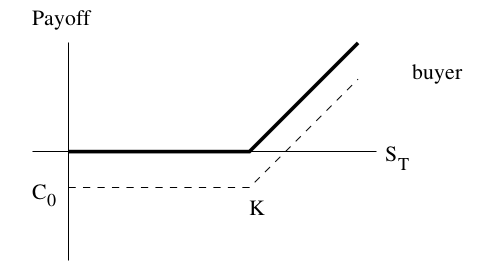
\includegraphics[width=1\linewidth]{Buyer_call} 
		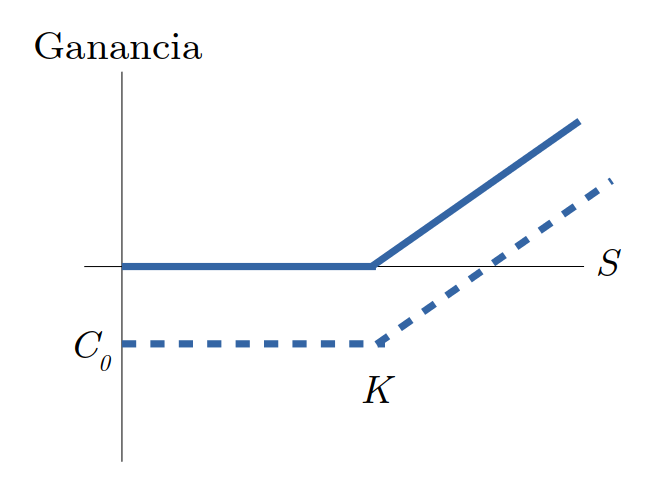
\includegraphics[width=1\linewidth]{Buyer_call_mio} 
		\caption*{Propietario}
		%\label{fig:subim1}
	\end{minipage}
	\begin{minipage}{0.5\textwidth}
		%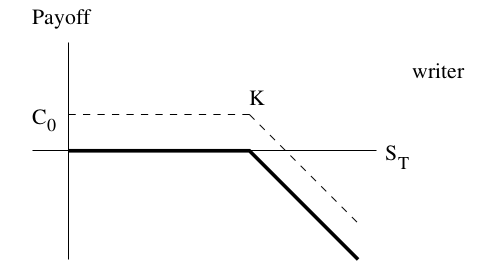
\includegraphics[width=1\linewidth]{Writer_call}
		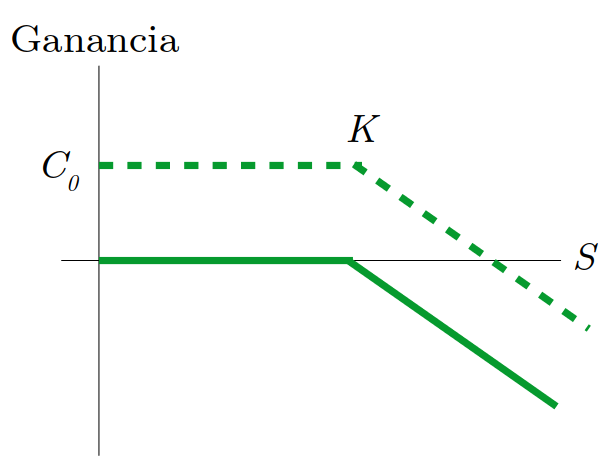
\includegraphics[width=1\linewidth]{Writer_call_mio}
		\caption*{Vendedor}
		
		%\label{fig:subim2}
	\end{minipage}
	\caption{Ganancia opción \textit{call}.}
	\label{graphCall}
\end{figure}

\begin{figure}[h!]
	
	\begin{minipage}{0.5\textwidth}
		\centering
		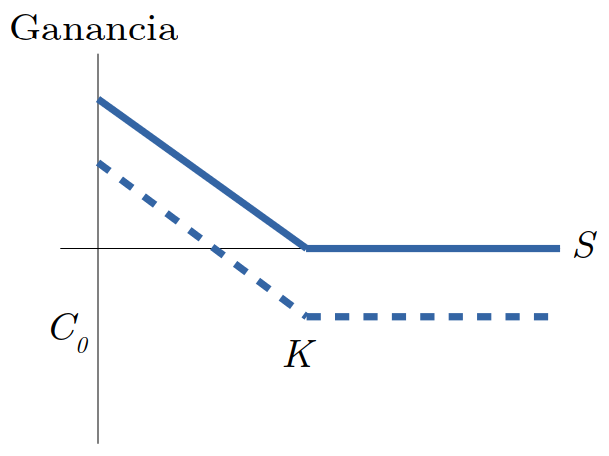
\includegraphics[width=1\linewidth]{Buyer_put_mio} 
		\caption*{Propietario}
		%\label{fig:subim1}
	\end{minipage}
	\begin{minipage}{0.5\textwidth}
		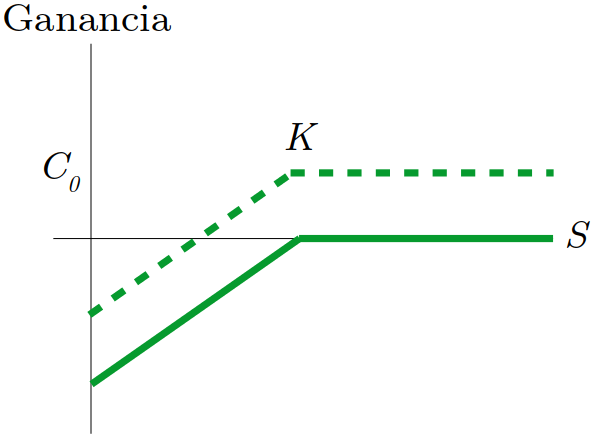
\includegraphics[width=1\linewidth]{Writer_put_mio}
		\caption*{Vendedor}
		%\caption{Tras cuatro iteraciones.}
		
		%\label{fig:subim2}
	\end{minipage}
	\caption{Ganancia opción \textit{put}.}
	\label{graphPut}
\end{figure} 
Uno de los problemas más importantes es determinar de manera única el precio ``justo'' de una opción en un momento determinado para que ambas partes estén de acuerdo. Para más información acerca de conceptos financieros, se pueden consultar \cite{elliot1999mathematics} y el manual para universitarios publicado por la Comisión Nacional del Mercado de Valores.\\

\section{Primer teorema fundamental}
Una vez explicada de manera simplificada el contexto financiero debemos formalizar matemáticamente el modelo del mercado. Para ello, seguimos \cite{elliot1999mathematics}. Fijamos el conjunto de tiempos $ \mathbb{T} = \{0,1,\dots,T\}$ con $ T $ el instante en el que finaliza el modelado de nuestra actividad económica. También fijamos el espacio de probabilidad $ (\Omega, \mathcal{F}, P) $. Este espacio contiene todos los posibles estados del mercado. La información de la que disponen los inversores acerca de la estructura en cada momento $ t \in \mathbb{T}$ viene dada por una sucesión finita y creciente de sub-$ \sigma $-álgebras de $ \mathcal{F} $, $ \mathcal{F}_0 \subset \cdots \subset \mathcal{F}_T = \mathcal{F} $ con $ \mathcal{F}_0 $ trivial, es decir, contiene solamente conjuntos con medida 0 o 1. A este secuencia se le denomina filtración y se denota como $ \mathbb{F} = (\mathcal{F}_t)_{t \in \mathbb{T}} $. El sentido financiero de esta filtración es indicar la información conocida hasta el momento acerca de la evolución de los precios. Por ejemplo, si comenzamos a modelar nuestro mercado hoy, $ \mathcal{F}_0 $ nos aporta únicamente el valor actual. Sin embargo, mañana tendremos la información de los precios en ese momento junto con la obtenida hoy, por lo que es claro que $ \mathcal{F}_0 \subset \mathcal{F}_1  $. También es claro que al llegar al instante final tenemos toda la información acerca del modelo. Llamamos $ d  $ a la dimensión de nuestro mercado, es decir, el número de activos que manejamos. La evolución de los precios de los activos viene dada  por el proceso estocástico $ S = \{S^i_t:\hspace{1mm} t \in \mathbb{T},\hspace{1mm} i=0,\dots,d\} $ donde cada $ S^i_t $ es una variable aleatoria. Todos son activos con riesgos menos el marcado por $ 0 $. Asumimos que el proceso $ S_t^i $ es $ \mathcal{F}_t $-medible para $ i=0,\dots,d $, es decir, se adapta a la filtración $ \mathbb{F} $. Eso significa que para cada $ t \in \mathbb{T} $ se conocen los precios de cada activo hasta ese instante como se ha explicado anteriormente. En general, primero se escoge $ S $ y se toma $ \mathbb{F} $ como la filtración que genera. La tupla $ (\Omega, \mathcal{F}, P, \mathbb{F}, S) $ es la que modela nuestro mercado de valores. \\

El poder adquisitivo de una misma cantidad decrece con el tiempo, consideramos el factor de descuento (o de actualización) en el instante $ t $ dado por $ \beta_t < 1 $ y notamos al valor actual como $ \bar{S}_t = \beta_t S_t $. Sin pérdida de generalidad se puede asumir que $ S^0(0) = 1 $ por lo que podemos expresar todas las unidades en función a dicho valor. En ese caso, el factor $ \beta_t = 1/S^0_t $ es la cantidad de dinero que necesitamos para invertir en bonos en el instante 0 para tener una unidad en el instante $ t $. Podríamos considerar que tomar $ S^0(0) = 1 $  es una simple normalización de los precios. El factor de descuento se puede ver como $ \beta_t = (1+r)^{-t} $. Para entender esta fórmula podemos ver la situación contraria: calcular una cantidad con cierto intereses. De este modo, $ r $ representa el interés considerado o cómo aumentará el valor del dinero en el futuro. Así, el valor de una cantidad $ S $ en el futuro es $ (1+r)S $ considerando solo un paso o $ (1+r)^t S $ si consideramos varios. Por eso, al actualizar pasamos dicho término dividiendo y llegamos a la fórmula de $ \beta_t $ expuesta. Observemos que en ocasiones, como en el caso continuo, el papel de $ (1+r)^t $ es una función exponencial.\\

La cartera de inversión o portafolio para el instante $ t \in \mathbb{T} $ viene dada por la variable aleatoria $ d+1 $ dimensional $ \theta_t = (\theta_t^0,\dots,\theta_t^d) $. Cada $ \theta_t^i $ indica el número de activos del tipo $ i $ que tiene un inversor en el instante $ t $. El valor de la cartera viene determinado por $ V_t(\theta) $ donde
\[
V_0(\theta) = \langle \theta_1 , S_0\rangle, \hspace{2.5mm} V_t(\theta) = \langle \theta_t , S_t\rangle = \sum_{i=0}^{d} \theta_t^i S_t^i \text{ para } \hspace{0.5mm} t \in \mathbb{T}, t \geq 1.
\]
Cada inversor selecciona la cartera de inversión del instante $ t $ una vez se conocen los precios del momento anterior $ t-1 $. La estrategia de inversión $ \theta = \{\theta_t: \hspace{0.5mm}t=1,\dots,T\} $ es el conjunto de todas las carteras de inversión \textit{predecibles}. Decimos que una cartera $ \theta_{t} $ es predecible si depende solamente de los precios de los activos hasta el instante $ t-1 $. Cuando cada cartera de inversión $ \theta_{t+1} $ se puede financiar completamente con las ganancias o pérdidas actuales decimos que la estrategia es \textit{autofinanciada}, es decir, 
\begin{equation*}\label{selfinance}
\langle \theta_{t+1}, S_t \rangle = \langle \theta_{t}, S_t \rangle,
\end{equation*} Notamos $ \Delta X_t = X_t - X_{t-1} $ para cualquier función sobre $ \mathbb{T} $. Si una cartera es autofinanciada, escribimos la ganancia de una cartera de inversión entre los instantes $ (t-1,t] $ como 
\[
\Delta V_t(\theta) = \langle\theta_t, S_t \rangle - \langle\theta_{t-1}, S_{t-1}\rangle = \langle\theta_t, S_t \rangle - \langle\theta_{t}, S_{t-1}\rangle = \langle\theta_{t}, \Delta S_{t}\rangle.
\]
De este modo, la ganancia asociada a la estrategia $ \theta $ hasta el instante $ t $ viene dada por
\[
G_0(\theta) = 0, \hspace{2.5mm} G_t(\theta) = \langle\theta_{1}, \Delta S_{1}\rangle + \cdots + \langle\theta_{t}, \Delta S_{t}\rangle \text{ para } \hspace{0.5mm} t \in \mathbb{T}, t \geq 1.
\]
Vemos entonces que una estrategia es autofinanciada si, y solo si
\begin{equation}\label{selfinifonlyif}
V_t(\theta) = V_0(\theta) + G_t(\theta), \hspace{1mm} \forall t \in \mathbb{T}.
\end{equation}

Destacamos que todas la definiciones anteriores se pueden definir también en base a los valores actualizados $ \bar{S}_t $. \\

También es necesario imponer o aclarar una serie de suposiciones sobre nuestro modelo financiero:
\begin{enumerate}
	\item Ninguna de las transacciones conlleva un coste extra.
	\item Positividad: todos los precios son positivos, es decir,
	\[
	S_t^i > 0 \text{ para } t \in \mathbb{T},\hspace{1mm} i=0,\dots,d.
	\]
	\item Divisibilidad, liquidez y \textit{short selling} (venta en corto): el número de activos que posee un inversor puede ser cualquier valor real. Así,
	\[
	\theta_t^i \in \RR \text{ para } t \in \mathbb{T},\hspace{1mm} i=0,\dots,d.
	\]
	La divisibilidad hace referencia a que $ \theta_t^i $ puede ser una fracción. Claramente, no podemos tener, por ejemplo, media acción. Sin embargo, cuando estamos trabajando con un gran número de acciones podemos considerar que tienen cifras decimales para trabajar con números menores. El hecho de que tome valores en $ \RR $ también significa que podemos comprar o vender el número de acciones deseado, es decir, no imponemos ninguna restricción. Este hecho se conoce como liquidez. Claramente, en mercados reales sí existe dicha restricción en el volumen de las transacciones pero nosotros estamos trabajando con un modelo idealizado. Finalmente, cuando dichos valores son positivos decimos que el inversor tiene una posición larga o \textit{long position}. Si por el contrario estos son negativos, tiene una posición corta o \textit{short position}, por ejemplo, cuando vende algún tipo de bono. Estas acciones se suelen llevar a cabo, por ejemplo, en las denominadas ventas en corto o \textit{short selling} que se usan cuando se prevé que un determinado activo va a bajar de valor. Así, suponemos que tenemos una acción cuyo precio actual es 100 cuyo valor suponemos que va a disminuir. Antes de que baje más, la vendemos, es decir, tomamos una posición \textit{short}. Pasado un periodo de tiempo, la acción bajan a 70 por lo que tomamos una posición \textit{long} y las compramos de nuevo. De este modo, tenemos las misma cantidad de activos que al principio pero hemos obtenido un beneficio de 70. En estas operaciones también corremos el riesgo de perder dinero ya que es posible que el valor de los activos crezca en vez de disminuir. 
	
	\item Solvencia: el valor de todas las carteras de inversión debe ser siempre positivo,
	\[
	V_t (\theta) \geq 0\text{ para todo } t \in \mathbb{T}.
	\]
	En este caso, decimos que la cartera es \textit{admisible}. A la clase de estrategias autofinanciadas y admisibles la denotaremos como $ \Theta_a $.
	\item El espacio $ \Omega $ es finito, es decir, las variables aleatorias $ S_t^i $ no pueden tomar infinitos valores. Así, tenemos que $ \Omega = \{ \omega_1,\dots,\omega_n\} $.
\end{enumerate}

Ya tenemos el modelo financiero sobre el que vamos a trabajar. Exponemos ahora unos resultados que nos servirán posteriormente para probar el teorema principal del capítulo.
\bigskip
%% Parecido Prop 4.1 del otro libro Mathematics for finance
%% LEMMA 2.2.1
\begin{lemaBox}\label{2.2.1}
	Dada $ V_0 $ una función $ \mathcal{F}_0 $-medible y para $ d \in \NN  $ sean los procesos reales y predecibles $ \theta^1,\dots,\theta^d $, el único proceso predecible $ \theta^0 $ que convierte a $ \theta = (\theta^0,\theta^1,\dots,\theta^d) $ en una estrategia autofinanciada con valor $ V_0 (\theta)= V_0 $ viene dado por
	\[
	\theta^0_t = V_0 + \sum_{i=1}^{t-1}(\theta^1_i\Delta\bar{S}^1_i+\cdots+\theta^d_i\Delta\bar{S}^d_i) - (\theta^1_t\bar{S}^1_{t-1}+\cdots+\theta^d_t\bar{S}^d_{t-1}).
	\]
\end{lemaBox}
\begin{proof}
	Claramente $ \theta^0 $ es predecible. Para ver que la estrategia es autofinanciada, por \eqref{selfinifonlyif} solo necesitamos ver que $ \theta^0_t $ es la única solución predecible de la ecuación 
	\begin{equation*}
	\begin{split}
	\bar{V}_t(\theta) &= \theta^0_t + \theta^1_t\bar{S}^1_t+\cdots+\theta^d_t\bar{S}^d_t \\
	&= V_0 + \sum_{i=1}^{t}(\theta^1_i\Delta\bar{S}^1_i+\cdots+\theta^d_i\Delta\bar{S}^d_i)
	\end{split}
	\end{equation*}
\end{proof}
\bigskip
Introducimos ahora el concepto de \textit{viabilidad}, esencial para lo que sigue. Decimos que un mercado es viable si para toda estrategia admisible y autofinanciada no contiene ninguna oportunidad de arbitraje. La ausencia de arbitraje significa que si el valor inicial de una cartera de inversión es $ V_0(\theta) = 0 $ entonces $ V_T(\theta) = 0 $ con probabilidad 1 para toda $ \theta \in\Theta_a $. La viabilidad del mercado impone la siguiente restricción.

\bigskip
%% LEMMA 3.2.1
\begin{lemaBox}\label{3.2.1}
	Si el modelo de mercado es viable, las ganancias actualizadas a cualquier proceso predecible $ \hat{\theta} \in \RR ^d $ no pueden pertenecer a 
	\[
	C = \{Y \in \RR^n: Y_i \geq 0\text{ para } i=1,\dots,n \text{ y } \exists i \text{ tal que } Y_i > 0\}.
	\]
\end{lemaBox}
\begin{proof}
	En primer lugar vemos que $ C $ es el octante positivo de $ \RR^n $ sin el origen, que claramente es un cono y es convexo. La ausencia de arbitraje significa que para toda estrategia admisible $ \theta \in \Theta_a $ tal que $ V_0(\theta) = 0 $ entonces
	\[
	\bar{V}_t(\theta) = \bar{G}_t (\theta) \notin C.
	\]
	Por el lema \ref{2.2.1}, dados los procesos predecibles $ \hat{\theta} = (\theta^1, \dots,\theta^d) $, existe un único proceso real $ \theta^0 $ tal que $ \theta = (\theta^0, \theta^1,\dots, \theta^d) $ es autofinanciada y $ V_0(\theta) = 0 $. Las ganancias con los valores actualizados viene dada por
	\[
	\bar{G}_t(\hat{\theta}) = \sum_{j=1}^{t} \langle \theta_j, \Delta \bar{S}_j \rangle =   \sum_{j=1}^{t} \left( \sum_{i=1}^{d} \theta_j^i \Delta \bar{S}_j^i  \right).
	\]
	Supongamos que $ \bar{G}_t(\hat{\theta}) \in C $; si $ \beta_T $ denota el factor de descuento en el instante $ T $,
	\[
	V_T(\theta) = \beta_T^{-1} \bar{V}_t(\theta) = \beta_T^{-1}(V_0 (\theta) + \bar{G}_t(\theta)) = \beta_T^{-1}\bar{G}_t(\theta).
	\]
	Vemos entonces que $ V_T(\theta) $ es no negativa y estrictamente positiva con probabilidad no nula, lo que contradice la viabilidad al existir arbitraje.
\end{proof}
\bigskip
Nuestro objetivo es caracterizar la viabilidad de un mercado en términos de los incrementos de $ \bar{S} $. Para ello son necesarias las martingalas.
\bigskip
\begin{definicion}
	Un proceso $ \mathbb{F} $-adaptado $ M = (M_t)_{t\in \mathbb{T}} $ es una $ ( \mathbb{F},P)$-mar\-tingala si $ E(|M_t|) < \infty $ para todo $ t \in \mathbb{T} $ y 
	\[
	E(M_{t+1}|\mathcal{F}_t) = M_t \textit{ para todo } t \in \mathbb{T}\setminus{T}.
	\]
	Si $ M = (M_t) $ es una martingala y $ \phi = (\phi_t)_{t\in \mathbb{T}} $ es un proceso predecible en $ (\Omega, \mathcal{F}, P, \mathbb{F}, S) $ entonces al proceso $ X = \phi \cdot M $ dado por
	\[
	X_0=0, \hspace{2mm}X_t = \phi_1\Delta M_1+\cdots+ \phi_t\Delta M_t \hspace{1.5mm} t \geq1
	\]
	se le denomina martingala transformada de $ M $ por $ \phi $.
\end{definicion}

Notamos que $ M $ es una martingala si, y solo, si
\[
E(\Delta M_{t+1} |\mathcal{F}_t ) = 0 \text{ para todo } t\in \mathbb{T}\setminus\{T\}.
\]
También es importante destacar que, por la linealidad de la esperanza, cualquier combinación lineal de martingalas es una martingala. \\

Que los precios en el mercado sigan una martingala no debe de ser extraño. Recordemos que para $ t \in \mathbb{T} $, $ \mathcal{F}_t $ indica la cantidad de información acerca de los precios de los activos hasta dicho momento. Por lo tanto, la esperanza condicionada solo nos indica que estamos calculando el valor esperado a partir de lo que conocemos hasta ahora. Además, para que el mercado sea ``justo'', dicho valor en el futuro debería ser, en media, el que tenemos ahora. \\

El siguiente resultado es meramente técnico y nos servirá posteriormente. 

\bigskip
%% THEOREM 2.3.5
\begin{teoremaBox}\label{2.3.5}
	Un proceso real $ M $ es una martingala si, y solo si, 
	\[
	E((\phi \cdot M)_t) = E(\sum_{i=1}^{t}\phi_i\Delta M_i) = 0, \hspace{1mm} \forall t \in \mathbb{T}\setminus\{0\}
	\]
	para todo proceso $ \phi $ predecible y acotado.
\end{teoremaBox}
\begin{proof}
	Si $ M $ es un martingala, también lo es la tranfomada $ X = \phi \cdot M $ y $ X_0 =0 $ ya que
	\[
	E(\Delta X_{t+1}|\mathcal{F}_t) = E(\phi_{t+1}\Delta M_{t+1}|\mathcal{F}_t) =  \phi_{t+1} E(\Delta M_{t+1}|\mathcal{F}_t) = 0.
	\] 
	Por ello, $ E((\phi \cdot M)_t) = 0 $ para todo $ t \geq 1 $ en $ \mathbb{T} $.
	Demostremos ahora la otra implicación. Para $ s > 0 $, sea $ A \in \mathcal{F}_s $ y definimos el proceso predecible $ \phi $ como $ \phi_{s+1} = 1_A $ y $ \phi_t = 0 $ para el resto de $ t\in \mathbb{T} $. Entonces, para $ t > s $ se tiene que
	\[
	0 = E((\phi \cdot M)_t) = E(1_A(M_{s+1}-M_s)).
	\]
	Como es cierto para todo $ A \in \mathcal{F}_s $, se cumple que $ E(\Delta M_{s+1} | \mathcal{F}_s) = 0 $ por lo que $ M $ es una martingala.
\end{proof}
\bigskip
Nos encontramos ahora un contexto general donde no asumimos que el modelo sea finito o que $ \mathbb{F} $ sea generada por $ S $. Supongamos que el proceso de los precios actualizados $ \bar{S} $ es una martingala bajo una probabilidad $ Q $, esto es:
\[
E_Q (\Delta \bar{S}^i_t | \mathcal{F}_{t-1}) = 0, \text{ para } t \in \mathbb{T}\setminus \{0\} \text{ e } i = 0,\dots,d,
\]
donde $ E_Q $ significa la esperanza respecto de la probabilidad (medida) $ Q $. Sea $ \theta \in \Theta_a $ una estrategia admisible tal que los procesos de los precios actualizados son integrables respecto a $ Q $. Por \eqref{selfinifonlyif} tenemos que:
\begin{equation*}
\begin{split}
\bar{V}_t(\theta) &= V_0(\theta) + \bar{G}_t(\theta) \\
&= \langle \theta_{1}, S_0 \rangle + \sum_{u=1}^{t} \langle \theta_{u}, \Delta \bar{S}_u \rangle \\
&= \sum_{i=1}^{d}(\theta_1^i S_0^i + \sum_{u=1}^{t} \theta_{u}^i \Delta \bar{S}_u^i).
\end{split}
\end{equation*}
Vemos entonces que $ \bar{V}(\theta) $ es una constante más una suma finita de martingalas transformadas, por lo que también es una martingala con valor inicial $ V_0 (\theta) $. Entonces, tenemos que: \[ E(\bar{V}_t (\theta)) = E(V_0 (\theta)) = V_0(\theta) .\] 
Esta situación imposibilita la existencia de arbitraje. Si sabemos de antemano que los procesos de los precios actualizados son integrables respecto a $ Q $, supongamos que $ V_0 (\theta) = 0$ y $ V_T (\theta) \geq 0$ casi seguramente (respecto a $ Q $). Como $ E_Q = (\bar{V}_t ( \theta)) = 0 $ se sigue que $ V_T(\theta) = 0$ casi seguramente (respecto a $ Q $). Esto sigue siendo verdadero casi seguramente para $ P $, demostrando que $ P $ y $ Q $ tienen los mismos conjuntos vacíos. Llegamos entonces a la siguiente definición:
\bigskip
\begin{definicion}
	Una probabilidad $ Q $ que sea equivalente a $ P $ como media $ (Q\sim P) $ es una medida martingala equivalente (EMM) para $ S $ si el proceso de los precios actualizados $ \bar{S} $ es una martingala bajo $ Q $ para la filtración $ \mathbb{F} $. Es decir, para cada $ i =0,\dots, d $ tenemos que $ \bar{S}^i $ es una $ (\mathbb{F},Q) $-martingala.
\end{definicion}
\bigskip
Todo lo presentado anteriormente, nos aporta el siguiente resultado que acabamos de demostrar:
\bigskip
\begin{proposicionBox}\label{martThenViab}
	Si existe una medida martingala equivalente para $ S $, entonces el modelo de mercado discreto es viable, es decir, no contiene ninguna oportunidad de arbitraje.	
\end{proposicionBox}
\bigskip
El recíproco de esta afirmación es cierto, tal y como exponemos en el siguiente teorema que es el objetivo final de este capítulo y en el que usaremos el teorema de la alternativa de Gordan en forma equivalente del teorema de separación establecido en el corolario \ref{coroSep}. Recibe el nombre de ``primer teorema fundamental de asignación de precios''.
\bigskip
\begin{teoremaBox}(Primer reorema fundamental de asignación de precios)\label{VIABLEiofEMM}
	Un modelo de mercado discreto es viable si, y solo si, existe una medida de martingala equivalente para $ S $.
\end{teoremaBox}
\begin{proof}
	Ya sabemos por la proposición \ref{martThenViab} que la existencia de una medida de martingala equivalente garantiza la viabilidad del modelo por lo que solo tenemos que probar la otra implicación. \\
	
	Suponemos entonces que el modelo es viable. Necesitamos construir una medida $ Q \sim P $ en la que los precios son martingalas relativas a la filtración $ \mathbb{F} $. Sea $ C $ es el cono convexo de todas las variables aleatorias reales $ \phi $ en $ (\Omega, \mathcal{F}) $ tales que $ \phi(\omega) \geq 0 $ casi seguramente y $ \phi(\omega_i) > 0 $ para al menos un $ \omega_i = \Omega = \{\omega_i,\dots, \omega_n \} $. Asumimos $ p_i = P(\{\omega_i\}) > 0 $. Por el lema \ref{3.2.1}, hemos visto que para un mercado viable debemos tener $ \bar{G}_t(\hat{\theta}) \notin C$ para todos los procesos predecibles $ \hat{\theta} \in  \RR^d $. Por otro lado, el conjunto definido por tales ganancias 
	\[
	L = \{\bar{G}_t(\hat{\theta}):\hspace{0.5mm} \hat{\theta}=(\theta^1,\dots,\theta^d),\text{ con } \theta^i \text{ predecible para } i=1,\dots,d \},
	\]
	es un subespacio vectorial del espacio de todas las funciones reales y  $ \mathcal{F} $-medibles en $ \Omega $. Como $ L $ y $ C $ son disjuntos, podemos separar $ L $ y el subconjunto compacto de $ C $ definido como $ K =\{X\in C: \hspace{0.5mm} E_P(X) = 1\} $ gracias al corolario \ref{coroSep}. Sea $ \xx^0 \in \RR^d $ el elemento que proporciona dicho resultado. Tomamos $ \xi_i = (0,\dots,\frac{1}{p_i},\dots,0) $ para $ i \leq n $. Vemos que $ E_P(\xi_i) = \frac{p_i}{p_i} = 1$ por lo que $ \xi_i \in K $ y $ \langle \xx^0, \xi_i \rangle = \frac{x^0_i}{p_i} > 0$. Por ello, $ x^0_i > 0$ para todo $ i=1,\dots,n $.
	
	Definimos ahora el funcional lineal $ g(\xx) = \frac{\langle \xx^0, \xx\rangle}{\alpha} $ donde $ \alpha = \sum_{i=1}^{n} x^0_i$. Sea $ p^* \in \RR^d$ un vector con $ p^*_i = \frac{x_i^0}{\alpha} $ por lo que $ \sum_{i=1}^{n} p^*_i = 1 $. Usamos el vector $ p^* $ para inducir una probabilidad $ P^* $ en $ \Omega = \{\omega_1,\dots,\omega_n\} $ haciendo $ P^*(\{\omega_i\}) = p^*_{i} > 0 $. Veamos que $ P^* $ es la martingala equivalente deseada. En efecto, sea $ E^*(\cdot) $ que denota la esperanza relativa a $ P^* $. Nuevamente, por el corolario \ref{coroSep}, tenemos que $ g(\xx) = \frac{1}{\alpha}\langle \xx^0,\xx\rangle = 0$ para todo $ \xx\in L $. En particular, esta situación se da para  para $ \bar{G}_T (\hat{\theta}) $ con $ \hat{\theta}=(\theta^1,\dots,\theta^d) $ un vector de procesos predecibles por lo que.
	\[ E^*(\bar{G}_T (\hat{\theta})) = 0.\]
	Hemos conseguido una estrategia auto-financiada $ \theta $ con $ V_0(\theta) = 0 $. Como $ \bar{V}_t (\theta) = V_0(\theta) + \bar{G}_T (\theta)$, implica que $ E^*(\bar{V}_t (\theta)) = 0 $ para cada $ \theta $. Por el lema \ref{2.2.1} podemos generar tal $ \theta $ para cada proceso predecible de $ n $  dimensiones. En particular, lo podemos hacer para $ (0,\dots, \theta^i,\dots,0) $ donde $ i\leq n $. Por lo tanto
	\[
	E^*(\sum_{t=1}^{T}\theta_t^i\Delta \bar{S}^i_t) = 0
	\]
	se da para cada proceso predecible y acotado $ (\theta^i)_{i=1,\dots,T} $. El teorema \ref{2.3.5} implica que cada $ S^i $ es una martingala bajo $ P^* $. Por ello, $ P^* \sim P $.
\end{proof}
\bigskip
\input{capitulos/aplicación.tex}

\chapter{Conclusiones y vías futuras}
Los objetivos que nos marcamos en la propuesta inicial se han alcanzado satisfactoriamente. Es más, se ha realizado una incursión no prevista en la teoría minimax de manos de los teoremas de la alternativa. Ello ha permitido obtener una visión completa de las técnicas y aplicaciones de los teoremas de la alternativa.
%% Incluir en la bibliografía las referencias no citadas
\nocite{*}
% \bibliographystyle{alpha-es}
% \bibliography{bibliografia/bibliografia}
\begin{thebibliography}{X}
	\bibitem{borwein} J.M. Borwein, A.S. Lewis, \textsl{Convex analysis and nonlinear optimization: theory and examples}, Second Edition, CMS Books in Mathematics/Ourrages Mathématiques de la SMC 3, Springer, New York, 2006.
	
	\bibitem{elliot1999mathematics} R.J. Elliot, R.E. Kopp, \textsl{Mathematics of financial markets}, Second Edition, Springer Finance, New York, 2005.
	
	\bibitem{giorgi2004mathematics} G. Giorgi, A. Guerraggio, J. Thierfelder, \textsl{Mathematics of optimization: smooth and nonsmooth case}, Elsevier Science B.V., Amsterdam, 2004.
		
	\bibitem{König1} H. König, \textsl{Über dans von Neumannsche minimax-theorem}, Archiv der Mathematik 19(1968), 482-487.
	
	\bibitem{König2} H. König, \textsl{Sublinear functionals and conical measures}, Archiv der Mathematik 77(2001), 56-64.
	
	\bibitem{mo} S. Mazur, W. Orlicz, \textsl{Sur les espaces métriques linéaires II}, Studia Mathematica 13(1953), 137-179.

	\bibitem{schechter1996handbook} E. Schechter,
	\textsl{Handbook of analysis and its foundations}, Academic Press, Inc., San Diego, CA, 1999.
	
	\bibitem{Simons2008} S. Simons, \textsl{From Hahn-Banach to monotonicity}, 2nd edition, Lectures notes in Mathematics 1693, Springer, New York, 2008.
	
\end{thebibliography}

%\bibliographystyle{apalike-es}
%\bibliography{bibliografia/bibliografia}
%
%\input{capitulos/03_Planificacion}
%
%\input{capitulos/04_Analisis}
%
%\input{capitulos/05_Diseno}
%
%\input{capitulos/06_Implementacion}
%
%\input{capitulos/07_Pruebas}
%
%\input{capitulos/08_Conclusiones}
%
%%\chapter{Conclusiones y Trabajos Futuros}
%
%
%%\nocite{*}
%\bibliography{bibliografia/bibliografia}\addcontentsline{toc}{chapter}{Bibliografía}
%\bibliographystyle{miunsrturl}
%
%\appendix
%\input{apendices/manual_usuario/manual_usuario}
%%\input{apendices/paper/paper}
%\input{glosario/entradas_glosario}
% \addcontentsline{toc}{chapter}{Glosario}
% \printglossary

\end{document}
